\documentclass[11pt, a4paper, german]{article}
\usepackage[utf8]{inputenc}
\usepackage[ngerman]{babel}
\usepackage{amsmath}
\usepackage{amsthm}
\usepackage{amsfonts}
\usepackage{amssymb}
\usepackage{color}
%\usepackage{algorithmicx}
%\usepackage[compatible]{algpseudocode}
\usepackage{algorithm}
%\usepackage{algorithmic}
\usepackage{algpseudocode}
\usepackage{makeidx}
\usepackage{graphicx}
\usepackage{tabularx}
\usepackage{ulem}
\usepackage{bbm}
\usepackage{BA_Titelseite}
\usepackage{bm}
\usepackage[colorlinks=true, pdfborder={0 0 0}, linkcolor=black, citecolor=magenta]{hyperref}
\bibliographystyle{unsrt}



%Namen des Verfassers der Arbeit
\authornew{Boris Prochnau}

%Geburtsdatum des Verfassers
\geburtsdatum{22. Dezember 1989}
%Gebortsort des Verfassers
\geburtsort{Tartu}
%Datum der Abgabe der Arbeit
\date{\today}

%Name des Betreuers
% z.B.: Prof. Dr. Peter Koepke
\betreuer{Betreuer: Prof. Dr. Anton Bovier}
%Name des Instituts an dem der Betreuer der Arbeit tätig ist.
%z.B.: Mathematisches Institut
\institut{Institut für Angewandte Mathematik}
%Titel der Bachelorarbeit
\title{Simulation einer stochastischen Populationsdynamik}
%Do not change!
\ausarbeitungstyp{Bachelorarbeit Mathematik}

\theoremstyle{plain}
\newtheorem{satz}{Satz}[section]
\newcommand{\eps}{\ensuremath{\varepsilon}}
\newcommand{\tvec}[2]{\begin{pmatrix}#1\\#2\end{pmatrix}}
\newcommand{\trvec}[3]{\begin{pmatrix}#1\\#2\\#3\end{pmatrix}}


\begin{document}


\maketitle
\setcounter{tocdepth}{2}
\tableofcontents


\clearpage
\section{Einleitung}
Diese Bachelorarbeit behandelt die Entwicklung eines Programms zur Simulation einer Populationsdynamik. Dazu wird erst ein grundlegendes Modell vorgestellt, welches den zu simulierenden BPDL-Prozess beschreibt. Darüber hinaus wird das Programm auch in der Lage sein die Approximation von Grenzwertprozessen zu simulieren, die aus dem BPDL-Prozess gewonnen werden. Dazu zählt auch der sogenannte "{}TSS-Prozess"{}. Die Simulation einer Approximation des "{}TSS-Prozesses"{} ist besonders interessant und wird in Kapitel 3 eingeführt und in Kapitel 7 genauer beschrieben. Alle Simulationen sollen auf demselben Modell basieren.\\
Jedes Lebewesen einer Population (z.B. Pflanzen, Zellen, Tiere) wird durch ein Merkmal beschrieben. Diese Merkmale erzeugen Dynamik in der Population, in dem sie z.B. Größe, Essensaufnahme, Fortpflanzungsrate oder Konkurrenz zu anderen Merkmalen angeben.\\
In unserem Modell besteht ein Merkmal aus einer asexuellen Fortpflanzungsrate und zwei Todesraten. Die Todesraten bestehen aus einer natürlichen Todesrate und einer Todesrate, die durch Wettbewerb zu jedem anderen Lebewesen entsteht. Man bemerkt schon, dass ein Individuum in diesem Modell nur sterben, töten (durch Wettbewerb) oder sich fortpflanzen kann. Da die wettbewerblichen Todesraten der Individuen von der Populationsgröße abhängen, ist die resultierende Dynamik nicht trivial und ihr Studium von besonderem Interesse.\\
Des Weiteren umfasst das Modell eine Mutationswahrscheinlichkeit welche sich nicht auf bereits in der Population lebende Wesen, sondern auf neugeborene Individuen bezieht.\\
Da die Entwicklung der Population, und nicht die der Individuen, das Ziel unserer Simulation ist (im Gegensatz zu \cite{fournier2004microscopic}), simulieren wir viele Individuen auf wenige Merkmale verteilt. Deshalb wird man im simulierten Prozess zwar Tode und Geburten in Merkmalen verfolgen können, aber nicht welches Individuum dieses Ereignis auslöst. Der Übergang zu dieser Sichtweise wird näher im 2. Kapitel beschrieben.\\
Hauptsächlich wird in dieser Arbeit beschrieben, wie sich dieses Modell und seine Eigenschaften auftrennen oder zusammenfassen lassen um möglichst effizient und sicher ein Programm zur Simulation eines entsprechenden Prozesses zu implementieren. Dabei wird oft auf moderne Methoden zurückgegriffen, die eine möglichst unabhängige Strukturierung der Schritte während eines Ablaufs voraussetzen.\\
Schließlich wird auch beschrieben, was eine Simulation leisten kann, sollte und was diese Simulation tatsächlich tut. Z.B. sollte die graphische Darstellung des Prozesses die Möglichkeit bieten, beobachten zu können, ob sich ein Merkmal unter anderen durchsetzten kann, es einen stabilen Zustand annimmt oder dem Tod entgegen strebt.


\clearpage
\section{Modell}
Das verwendete Model wurde in \cite{Bolker_Spatial_moment,Bolker1997179,raey_Dieckmann_Law} eingeführt. Bei asexueller Vermehrung nutzt das Modell die drei grundlegenden Mechanismen von Darwins Evolutionslehre: Vererbung, Variation (Mutationen) und Selektion durch Wettbewerb, um eine Menge von Merkmalen für Individuen zu beschreiben. Diese bestimmen die Fähigkeit des Individuums zu überleben und sich fortzupflanzen. Der daraus resultierende zeitstetige Sprung-Prozess wird BPDL-Prozess (nach Bolker, Pacala, Dieckmann und Law) genannt.\\
Ziel ist es, zwei spezielle BPDL-Grenzwert-Prozesse zu simulieren.
	\subsection{Grundlagen}
	Sei $ X $ der endliche diskrete Raum der Merkmale. Jedes Individuum hat genau ein solches Merkmal $ x \in X $, wodurch es vollständig charakterisiert ist. Es ist hilfreich sich X als Indexmenge $ X = \{1,\dots, n\} $ vorzustellen, die abgezählte Merkmale enthält. Das entspricht auch der Interpretation von X aus Sicht der Simulation. Der Übersicht halber werden Elemente aus $ X $ jedoch mit $ x,y \in X $ angesprochen. Ein allgemeineres Modell findet sich in \cite{raey}.\\
	Für jedes Individuum mit Merkmal $ x \in X $ gilt:
	\begin{itemize}
		\item Jedes Individuum kann sich nur asexuell fortpflanzen oder sterben.
		\item Fortpflanzungs- und Todeszeitpunkte können durch sogenannte exponentielle Uhren beschrieben werden (wie in \cite[S. 3]{fournier2004microscopic}). Diese Uhren haben exponentiell verteilte Weckzeiten. Durch die Gedächtnislosigkeit der Exponentialverteilung und wegen des Wettbewerbs können und müssen alle Uhren nach dem ersten Klingeln neu gestellt werden. Durch den Einfluss des Wettbewerbs ist jede Todesrate abhängig von der Anzahl an Konkurrenten, die durch das zuerst eintretende Ereignis beeinflusst wird. 
		\item Bei einer Fortpflanzung kann eine Mutation auftreten d.h. die Fortpflanzung des Individuums mit Merkmal $ x \in X $ kann in der Geburt eines Individuums mit Merkmal $ y \in X $ resultieren. Die Häufigkeit dieser Ereignisse wird durch die Mutationswahrscheinlichkeit beschrieben.
	\end{itemize}
	Später wird deutlich, dass die Zurückstellbarkeit der Uhren entscheidend ist, um die Sichtweise von der Ebene des Individuums auf die der gesamten Population zu heben.\\
	Diese Todes- und Fortpflanzungsereignisse eines Individuums haben feste Raten, die das dazugehörige Merkmal beschreiben.\\
	
	\begin{tabular}{r p{26em}}
		$ b(x) $: & Ist die Geburtenrate durch ein Individuum mit Merkmal $ x $.\\
		$ d(x) $: & Ist die natürliche Todesrate. Im Folgenden wird stets vorausgesetzt, dass ein Merkmal überlebensfähig ist. Also $ b(x) - d(x) > 0 $.\\
		$ c(x, y) $: & Ist die Todesrate durch Wettbewerb, die ein Individuum $ y $ auf $ x $ ausübt. Diese Interpretation orientiert sich an \cite{raey}, während u.a. in \cite{Champagnat20061127} ein symmetrischer Wettbewerbskern verwendet wird. Im Gegensatz zu vorher kann der Wettbewerb ein konkurrierendes Merkmal zum Aussterben zwingen.\\
		$ \mu $: & Ist die Mutationswahrscheinlichkeit "{}auf die Nachbarn"{} mit je $ \frac{\mu}{2} $ pro Nachbar. \\
	\end{tabular}\\

	Alle erwähnten Raten sind wie in \cite{fournier2004microscopic} endlich und positiv. \\
	Schließlich lassen sich durch das Superpositionsprinzip der Exponentialverteilung die beiden Todesraten zu einer gemeinsamen Todesrate zusammenfassen oder die arteigene Geburtenrate beschreiben.\\
	
	\begin{tabular}{ r p{18em} }
		$ b(x) \cdot (1 - \mu) $ & Ist die arteigene Geburtenrate eines Individuums mit Merkmal $ x $, also mutationsfreie Geburten.\\
		$ d(x) + \sum_{i=1}^{N_t} c(x, x_i) $ & Ist die gesamte Todesrate eines Individuums mit Merkmal x (mit $ N_t \hat{=} $ \#Individuen zur Zeit t mit Merkmal $ x $ und $ x_i $ das Merkmal des i-ten Individuums).\\
		$ d(x) + \sum_{y \in X} c(x,y) \cdot n_t(y) $ & Ist auch die gesamte Todesrate, diesmal jedoch über die Merkmale summiert, mit $ n_t(x) \hat{=} \text{\#Individuen}$ zur Zeit t mit Merkmal $ x $.
	\end{tabular}\\
	
	Im Unterschied zu \cite{Champagnat20061127} sind wir an der Entwicklung einer großen Population mit wenigen Merkmalen interessiert. Deswegen ist es unpraktisch weiterhin die Raten jedes Individuums zu berechnen.\\
	Die letzte Darstellung der Todesrate ist z.B. praktischer für die Betrachtung der Population durch den Fokus auf die Merkmale. Ähnlich können weitere Ereignisse zusammengefasst werden, so dass man z.B. eine Todesrate und eine arteigene Geburtenrate der Merkmale erstellen kann:
	
	\begin{itemize}
		\item Die \textbf{Fortpflanzungsrate} des Merkmals $ x $: 
		\[ \tilde{B}(x) = b(x) \cdot n_t(x) \]
		Diese beschreibt die Rate, mit der Fortpflanzungen innerhalb des Merkmals x stattfinden (nicht die Geburten innerhalb x!).\\
		\item Die arteigene Geburtenrate (\textbf{Wachstumsrate}) des Merkmals $ x $ ist von besonderem Interesse und ist das, womit wir folgend hauptsächlich arbeiten werden: 
		\begin{align*}
			B(x)  & = (1 - \mu) \cdot b(x) \cdot n_t(x)\\
				  & + \frac{\mu}{2} \cdot \underbrace{b(x+1) \cdot n_t(x+1)}_{\text{Mutation von rechts}} \cdot \mathbbm{1}_{x<n}\\
				  & + \frac{\mu}{2} \cdot \underbrace{b(x-1) \cdot n_t(x-1)}_{\text{Mutation von links}} \cdot \mathbbm{1}_{x>1}
		\end{align*}
		Hierbei ist zu beachten, dass: $ \sum_{x \in X} B(x)  = \sum_{x \in X} \tilde{B}(x)$, da die Mutationen von rechts und links per Teleskopsumme den Faktor $ (1-\mu) $ ausgleichen.
		
		\item Die \textbf{Todesrate} des Merkmals $ x $:
		\[ D(x) = \underbrace{n_t(x) \cdot d(x)}_{\text{intrinsische Todesrate}} + \underbrace{n_t(x) \cdot \sum_{y=1}^{n} c(x,y) \cdot n_t(y)}_{\text{wettbewerbliche Todesrate}}  \]
	\end{itemize}
	Das entspricht zwei wesentlichen exponentiellen Uhren pro Merkmal: eine für Tod und eine für Geburt innerhalb des Merkmals.\\
	Für die Simulation ist eine Gesamtrate für das Eintreten eines Ereignisses praktischer. Auf diese Weise wird nur auf das Eintreffen einer Uhr gewartet.
	\begin{itemize}
		\item Ereignisrate des Merkmals $ x $ (Trait Rate):
		\[ TR(x) = B(x) + D(x) \]
		\item Totale Ereignisrate (Total Event Rate): 
		\[ TER = \sum_{x \in X} TR(x)\]
	\end{itemize}
	Mit der Totalen Ereignisrate gibt es eine Rate, die es erlaubt eine Zufallsvariable für das Eintreffen einer Variable zu ziehen. Anschließend ist es nur noch erforderlich (mit der Ziehung zweier weiterer Zufallsvairablen) festzustellen, welchem Merkmal welches Ereignis zukommt. Das Zusammenfassen der Raten vereinfacht es dem Programm, spätere Auswertungen und Funktionen bereitzustellen. So lässt sich z.B. aus der Geburtenrate (Wachstumsrate) eines ausgestorbenen Merkmals die Mutationsrate ablesen, ohne dass weitere Berechnungen gemacht werden müssen.\\
	
	\subsection{BPDL-Prozess}
	Eine auf diesem Modell basierende Population wird durch folgendes Punktmaß beschrieben:
	\[ \nu_t = \sum_{i=1}^{N_t} \delta_{x_i}, \quad x_i \hat{=} \text{Das Merkmal des i-ten Individuums} \]
	Es bildet Merkmale auf die Anzahl ihrer Repräsentanten ab.\\
	Mit Zeitpfaden ist $ \nu_t $ ein stochastischer Prozess, genauer ein Markov Sprung Prozess auf dem Maßraum:
	\[ \nu_t \in M(X) = \left\{ \sum_{i=1}^{m} \delta_{x_i}, m \in \mathbb{N}, x_1, \dots, x_n \in X \right\} \]
	Man erkennt leicht die Sprungeigenschaft:
	\[ \int_X 1 \text{ } \nu_t(dx) = N_t 
	\text{ und }
	\int_X \mathbbm{1}_y(x) \text{ } \nu_t(dx) = n_t(y) \]
	Normalerweise gehört zum Model des BPDL-Prozesses, dass die Mutationen auf einem beliebigen Merkmal (nicht nur den Nachbarn) landen können und der Raum der Merkmale nicht unbedingt diskret sein muss. Eine Mutationswahrscheinlichkeit hängt in diesem Fall vom Merkmal ab, also $ \mu(x) $. Der Mutant hat folglich Merkmal $ x + h $, wobei h eine zentrierte Zufallsvariable mit Dichte $ m(x,dh) $ auf $ (X - x) $ ist.
	Für einen solchen Prozess wäre der Generator definiert als:
	\begin{align*}
		L(\phi(\nu)) &= \int_{X} b(x)(1-\mu)[\phi(\nu + \delta_x) - \phi(\nu)]\nu(dx)\\
					  &+ \int_{X}\int_{\mathbb{R}^d} b(x) \cdot \mu [\phi(\nu + \delta_{x+z}) - \phi(\nu)] m(x,dz) \nu(dx)\\
				  	  &+ \int_{X} d(x)[\phi(\nu - \delta_x) - \phi(\nu)]\nu(dx)\\
				 	  &+ \int_{X} \left( \int_{X} c(x,y) \nu(dy) \right) [\phi(\nu - \delta_x) - \phi(\nu)]\nu(dx)
	\end{align*}
	mit $ \phi: M \to \mathbb{R} $. \\
	Dieser beschreibt die erwartete Änderung von $ \nu $ zur Zeit $ t $. Man erkennt, dass der Generator unabhängig von $ t $ ist, da er nur mit den zeitunabhängigen Parametern $ b, d, c, \mu $ konstruiert wurde. Natürlich ist der verwendete Prozess $ \nu_t $ abhängig von t, weshalb man $ \frac{d}{dt}\mathbb{E}\phi(\nu_t) = L\phi(\nu_t) $ schreiben kann.\\
	Mit unserem diskreten Raum X und der konstanten Mutationswahrscheinlichkeit zu Nachbarn vereinfacht sich der Generator. Der für unser Modell angepasste Generator hat somit folgende Form:
	\begin{align}
	\begin{split}
		L(\phi(\nu)) &= \sum_{x \in X} b(x)(1-\mu)[\phi(\nu + \delta_{x}) - \phi(\nu)] \cdot n(x)\\
		&+ \sum_{y \sim x}b(x) \cdot \frac{\mu}{2} \cdot 
 [\phi(\nu + \delta_{y}) - \phi(\nu)] \cdot n(x)\\		 
		&+ \sum_{x \in X} \left(d(x) + \sum_{y \in X} c(x,y) \cdot n(y)\right)[\phi(\nu - \delta_{x}) - \phi(\nu)] \cdot n(x) \label{GeneratorDiskret}
	\end{split}
	\end{align}
	mit $ \phi: M \to \mathbb{R} $.\\



\section{Eigenschaften des BPDL-Prozesses}
In diesem Kapitel werden Eigenschaften des Prozesses näher untersucht, die später bei der Simulation sichtbar sein sollen. Zunächst wird dabei die Normalisierung eingeführt, die es erleichtert Aussagen über das erwartete Verhalten des Prozesses bzw. der Population zu machen. 

	\subsection{Normalisierung des BPDL-Prozesses}
	Wie schon zuvor erwähnt ist es für uns wichtig, die Tode und Geburten nicht auf der Ebene des Individuums, sondern der gesamten Population zu betrachten. Dazu wird die LPA (Large Population Approximation) Normalisierung aus \cite{fournier2004microscopic} eingeführt.\\
	Hierfür wird der Prozess mit einem Parameter K skaliert und es ergibt sich eine neue Zufallsvariable:
	\[ \nu_t^K := \frac{1}{K} \nu_t \]
	Um für $ \nu_t^K $ dasselbe Verhalten wie für $ \nu_t $ zu erhalten, müssen einige Anpassungen vorgenommen werden.\\
	Zunächst wird die Anfangsgröße $ n_0^K $ der Population proportional zu K ge\-wählt.
	Die Raten für Geburten und natürliche Tode der Individuen bleiben unverändert. Da die Populationsgröße jedoch quadratisch in die Wettbewerbsrate einfließt, sollte $ c_K(x,y) = \frac{c(x,y)}{K} $ gelten, da sonst die K-fach erhöhte Population mit einem intensiven Aussterben den Vergleich verfälschen würde. \\
	Ein Beispiel für eine LPA-Normalisierung sieht folgendermaßen aus:
	\begin{figure}[H]
		\centering
		\begin{minipage}{1\textwidth}
		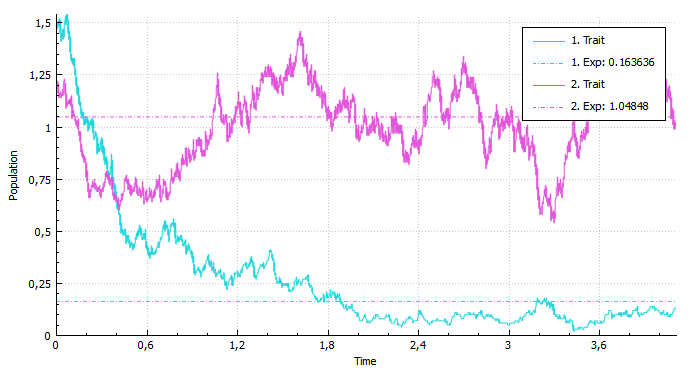
\includegraphics[width=0.5\linewidth]{./Pictures/LPANormalisierungK100}
		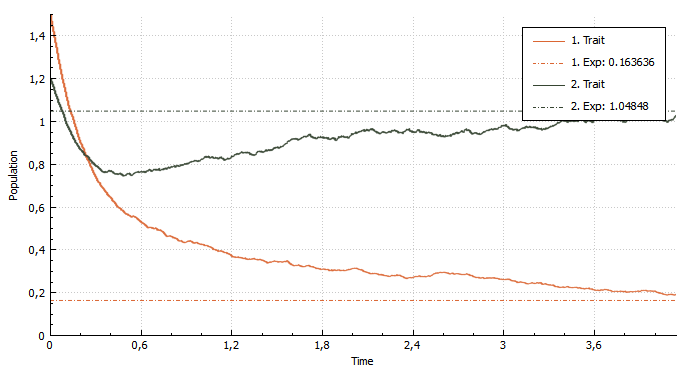
\includegraphics[width=0.5\linewidth]{./Pictures/LPANormalisierungK10000}
		\end{minipage}
		\caption[LPAK100]{LPA Normalisierung mit K=100 und K = 1000}
		\label{LPA-Normalisierung K=100_1000}
	\end{figure}
	Was bereits in beiden Abbildungen auffällt, ist dass die Population für kleine K fast sofort aussterben würde, weil die Merkmale sich auf ein gefährlich geringes Gleichgewicht einpendeln wollen.\\
	Für den Prozess $ \nu_t^K $ ändert sich der Generator ganz einfach zu:
	\begin{align*}
		L^K(\phi(\nu^K)) &= \int_{X} b(x)(1-\mu)\left[\phi\left(\nu^K + \frac{\delta_x}{K}\right) - \phi(\nu^K)\right]K\nu^K(dx)\\
			  &+ \int_{X}\int_{\mathbb{R}^d} b(x) \cdot \mu \left[\phi\left(\nu^K + \frac{\delta_{x+z}}{K}\right) - \phi(\nu)\right] m(x,dz) K \nu^K(dx)\\
		  	  &+ \int_{X} d(x)\left[\phi\left(\nu^K - \frac{\delta_x}{K}\right) - \phi(\nu^K)\right]K\nu^K(dx)\\
		 	  &+ \int_{X} \left( \int_{X} c_K(x,y) K \nu^K(dy) \right) \left[\phi(\nu^K - \frac{\delta_x}{K}) - \phi(\nu^K)\right]K\nu^K(dx)
	\end{align*}
	und in unserem Fall zu:
	\begin{align}
	\begin{split}
			L^K(\phi(\nu^K)) &= \sum_{x \in X} b(x)(1-\mu)\left[\phi\left(\nu^K + \frac{\delta_x}{K}\right) - \phi(\nu^K)\right]K \cdot n(x)\\
			&+ \sum_{y \sim x}b(x) \cdot \mu \cdot 
		 \left[\phi\left(\nu^K + \frac{\delta_y}{K}\right) - \phi(\nu^K)\right]K \cdot n(x)\\		 
			&+ \sum_{x \in X} \left(d(x) + \sum_{y \in X} c_K(x,y) K \cdot n(y)\right)\\
			&\cdot \left[\phi\left(\nu^K - \frac{\delta_x}{K}\right) - \phi(\nu^K)\right]K \cdot n(x) \label{GeneratorDiskretK}
	\end{split}
	\end{align}

	\subsection{LPA für zwei Merkmale ohne Mutation}
	Falls mit $ K \to \infty $ auch $ n_0^K \to n_0 $ folgt, dann lässt sich beweisen, dass das System gegen ein deterministisches System konvergiert $ \nu_t^K \xrightarrow{K} n_t $. Exemplarisch gehen wir von einem Fall von zwei Merkmalen ohne Mutation aus, jedoch lässt es sich auch auf d Merkmale auch mit Mutation erweitern. Dieses Beispiel ist für den TSS-Fall besonders interessant.\\
	Ein solches deterministisches System muss folgende Differentialgleichung erfüllen:
	\begin{align}
	\begin{split}
		\dot{n}(x) &= n(x) \left( b(x) - d(x) - c(x,x) n(x) - c(x,y) n(y) \right), \quad n_0(x) = n_{0,x}\\
		\dot{n}(y) &= n(y) \left( b(y) - d(y) - c(y,y) n(y) - c(y,x) n(x) \right), \quad n_0(y) = n_{0,y} \label{Differentialgleichung}
	\end{split}
	\end{align}
	Um die Konvergenz zeigen zu können, verwenden wir ein Theorem aus \cite[Kapitel 11, Thm 2.1]{ethier2009markov}.\\
	Dafür wird zunächst erläutert, ob unser Modell die Bedingungen aus \cite{ethier2009markov} erfüllt. Zu diesem Zweck wird unser mutationsfreies Modell in eine passende Notation aus \cite{ethier2009markov} übersetzt.\\
	Sei $ l \in \{ \binom{1}{0}, \binom{-1}{0}, \binom{0}{1}, \binom{0}{-1} \} $ und $ \beta_l : \mathbb{R}^2 \to \mathbb{R}_+ $. Mit $ l $ kann man das Merkmal und Ereignis auffassen, während $ \beta_l $ eine Ratenfunktion ist, welche die Raten eines Ereignisses für ein Merkmal der Population darstellt.\\
	In unserem Fall kann allerdings nur einem Merkmal ein Ereignis widerfahren. Deswegen werden unsere $ l $ stets Einheitsvektoren sein, die auf das Merkmal verweisen, mit Vorzeichen, die auf das Ereignis deuten. Z.B. $ l = \binom{0}{-1} $ meint einen Tod im zweiten Merkmal.\\
	Da $ \beta_l $ eine Population als Vektor erwartet, werden wir unsere Population mit $ n_t = \binom{n_t(x)}{n_t(y)} $ beschreiben. Daraus ergibt sich für das $ \beta $ mit obigem Beispiel:
	\[ \beta_{\binom{0}{-1}}(n_t)  = \beta_{\binom{0}{-1}}\tvec{n_t(x)}{n_t(y)} = d(y) \cdot n_t(y) + \left(\sum_{x \in X} c(y,x)n_t(x)\right) \cdot n(y) \]
	Dementsprechend ist:
	\[ \beta_{\binom{1}{0}}(n_t)  = b(x)n_t(x) \]
	Diese Raten lassen sich auch für $ \nu_t^K $ formulieren \cite[Kapitel 11 - (1.12)]{ethier2009markov}:
\begin{align*}
	q_l: \frac{\mathbb{N}}{K} &\longrightarrow \mathbb{R}_+\\
	q_l: \nu_t^K &\longmapsto K\beta_l\left(\frac{\nu_t}{K}\right)
\end{align*}
	Daran erkennt man, dass sich auch die Wettbewerbsrate zu unserer verändert:
	\begin{align*}
		K\beta_{\binom{-1}{0}}\left(\frac{\nu_t}{K}\right) &= K \cdot d(y)\frac{\nu_t(y)}{K} +  K \cdot \left(\sum_{x \in X} c(y,x) \cdot \frac{n_t(x)}{K}\right) \cdot \frac{n_t(y)}{K}\\
		&= d(y) \nu_t(y) + \left(\sum_{x \in X} \frac{c(y,x)}{K} \cdot n_t(x)\right) \cdot n_t(y)\\
		&= d(y) \nu_t(y) + \left(\sum_{x \in X} \bm{c^K(y,x)} \cdot n_t(x)\right) \cdot n_t(y)
	\end{align*}
	Die vorherigen Übersetzungen lassen sich leicht anhand des Generators nachvollziehen, wobei unser Generator (\ref{GeneratorDiskret}), nur ohne Mutation, dasselbe ergeben soll wie: 
	\[ \sum_l \beta_l(n_t)(f(n_t + l) - f(n_t)) \]
	Als nächstes kommen wir zur Definition des $ F $, welche sich aus der Gleichung \cite[Kapitel 6 - (2.2)]{ethier2009markov} ergibt:
	\[ F(n_t) = \sum_l l \beta_l (n_t) \]
	Wenn man die Summe für $ l = \tvec{1}{0}, l = \tvec{-1}{0} $ betrachtet, so beschränkt man sich auf die erste Zeile der Funktion, also:
	\[ F(n_t)_1 = 1 \cdot \underbrace{b(x)n(x)}_{\beta_{\binom{1}{0}} (n_t)} +  (-1) \cdot ( \underbrace{d(x)n(x) + \sum_{y \in X} c(x,y)n(x))}_{\beta_{\binom{-1}{0}} (n_t)}, \]
	was mit (\ref{Differentialgleichung}) übereinstimmt. Also gilt $ F_k(n_t) = \dot{n}_t(x_k) $, wobei $ x_k \hat{=} \text{k-te} $ Merkmal.\\
	Kommen wir nun zu dem eigentlichen Theorem.
	
	\begin{satz}[\cite{ethier2009markov}, Kapitel 11 - Theorem 2.1]\label{Konvegenzsatz}
		Sei $ V \subset \mathbb{R}^2 $ kompakt,
		\begin{align}
			\sum_l |l| \sup_{n_t \in V} \beta_l(n_t) < \infty \label{RatenEndlich}
		\end{align}
		und es existiert ein $ M_V > 0 $, sodass
		\begin{align}
			|F(n_t) - F(\tilde{n}_t)| \le M_V|n_t - \tilde{n}_t|, \qquad n_t, \tilde{n}_t \in V \label{Lipschitz}
		\end{align}
		Angenommen $ \nu_t^K $ erfüllt \cite[Kapitel 11 - (2.3)]{ethier2009markov} und $ \lim\limits_{K \to \infty} \nu_0^K = n_0 $, und n erfüllt
		\begin{align}
			n_t = n_0 + \int_{0}^{t} F(n_s) ds, \qquad t \ge 0 \label{Integralgleichung}
		\end{align}
		Dann gilt für jedes $ t > 0 $,
		\begin{align}
			\lim\limits_{K \to \infty} \sup_{s \le t} | \nu_t^K - n_t | = 0 \quad f.s. \label{Kovergenzbehauptung}
		\end{align}
	\end{satz}
	
	Es bleibt also zu zeigen, dass unser Modell die Bedingungen aus Satz \ref{Konvegenzsatz}, bzw. aus \cite[Kap. 11 - \textbf{Theorem 2.1}]{ethier2009markov} erfüllt.

	\begin{satz}
		Unser mutationsfreies Modell erfüllt die Bedingungen von \cite[Kap. 11 - \textbf{Theorem 2.1}]{ethier2009markov}.
	\end{satz}
	
	\begin{proof}
		Wir gehen zunächst von einer dimorphen Population $ X = \{x,y\} $ aus. Seien
		\[ n_1 = \tvec{n_1(x)}{n_1(y)}, \quad n_2 = \tvec{n_2(x)}{n_2(y)} \]
		zwei Lösungen der Differentialgleichung
		\begin{align}
		\begin{split}
		F(n) = \tvec{\dot{n}(x)}{\dot{n}(y)} =  \tvec{n(x)(b(x)-d(x)-c(x,x)n(x)-c(x,y)n(y))}{n(y)(b(y)-d(y)-c(y,y)n(y)-c(y,x)n(x))}\label{nDGL}
		\end{split}
		\end{align}
		ausgewertet zu einem Zeitpunkt $ s \in \mathbb{R}_{+} $.\\
	
		\textit{Bedingung (\ref{RatenEndlich})} bzw. \cite[Kapitel 11 - \textbf{Thm 2.1} (2.6)]{ethier2009markov} zu prüfen ist in unserem Fall sehr einfach.
		Unser Merkmalsraum und die verwendeten Raten sind endlich. Damit liegt stets eine endliche Stumme über endliche Raten vor, die natürlich wieder endlich ist. Das gilt für jedes $ n_t \in V $, da wir wie in \cite{fournier2004microscopic}, nur endliche Raten zulassen.\\
	
		\textit{Bedingung (\ref{Lipschitz})} bzw. \cite[Kapitel 11 - \textbf{Thm 2.1} (2.7)]{ethier2009markov} fordert
		\[ \left| F\tvec{n_1(x)}{n_1(y)} - F\tvec{n_2(x)}{n_2(y)} \right| < M_V \left| \tvec{n_1(x)}{n_1(y)} - \tvec{n_2(x)}{n_2(y)} \right|, \quad M_V \in \mathbb{R}_{+} \]
		für $ n_1, n_2 \in V $. Es ist klar, dass
		\begin{align}
		\begin{split}
			|n_1(x) - n_2(x)| \le |n_1 - n_2|\\
			|n_1(y) - n_2(y)| \le |n_1 - n_2| \label{epsAbsch}
		\end{split}
		\end{align}
		Falls es ein $ c_V \in \mathbb{R}_{+} $ gibt mit
		\begin{align}
		\begin{split}
			|F(n_1)_1 - F(n_2)_1| &\le |n_1 - n_2| \cdot c_V\\
			|F(n_1)_2 - F(n_2)_2| &\le |n_1 - n_2| \cdot c_V, \label{BeweisLipschitz}
		\end{split}
		\end{align}
		so folgt wegen 
		\begin{align}
		\begin{split}
			|F(n_1) - F(n_2)| &= \sqrt{(F(n_1)_1 - F(n_2)_1)^2 + (F(n_1)_2 - F(n_2)_2)^2}\\
			&\le \sqrt{(|n_1 - n_2| \cdot c_V)^2 + (|n_1 - n_2| \cdot c_V)^2}\\
			&= |n_1 - n_2| \cdot \underbrace{\sqrt{2} \cdot c_V}_{< \infty} = |n_1 - n_2| \cdot M_V \Rightarrow (\ref{Lipschitz})
			\label{epsBehauptung}
		\end{split}
		\end{align}
		Also bleibt nur noch (\ref{BeweisLipschitz}) zu prüfen. Dabei wird benötigt, dass $ |n_1(x)| + |n_2(x)| $ beschränkt ist. Das ergibt sich aus der Voraussetzung, dass $ V $ kompakt ist und $ n_1, n_2 \in V $ gewählt wurden. Diese Wahl ist für unser Modell sinnvoll, weil unsere Population mit einer endlichen Anfangsbedingung startet und bis zu einem festen Zeitpunkt $ t > 0 $ stets endliche Werte annimmt. Die Endlichkeit zu jedem Zeitpunkt $ t > 0 $ kann dadurch begründet werden, dass unsere Population durch eine identische ohne Todesraten zu jedem Zeitpunkt von dieser beschränkt wäre (also $ n_t(x) = b(x) \cdot t $).\\
		Für $ F_1 $ und $ F_2 $ ist dabei das Vorgehen analog, daher wird nur $ F_1 $ vorgestellt:\\
		\begin{align*}
			|F(n_1)_1 - F(n_2)_1| & = |(n_1(x) - n_2(x))(b(x) - d(x)) \\
			& - ((n_1(x))^2 - (n_2(x))^2) \cdot c(x,x)\\
			& - ((n_1(y))^2 - (n_2(y))^2) \cdot c(x,y) |\\
			& \le  |\underbrace{(n_1(x) - n_2(x))}_{ \le |n_1 - n_2|}(b(x) - d(x)) |\\
			& + | (n_1(x) - n_2(x))(n_1(x) + n_2(x)) \cdot c(x,x) | \\
			& + | (n_1(y) - n_2(y))(n_1(y) + n_2(y)) \cdot c(x,y) |\\
			& \le |n_1 - n_2| \cdot | b(x) - d(x) | \\
			& +  |n_1 - n_2| \cdot |\underbrace{n_1(x) + n_2(x)}_{\text{beschränkt}}| c(x,x) \\
			& + |n_1 - n_2| \cdot | n_1(y) + n_2(y) | \cdot c(x,y)\\
			& \le |n_1 - n_2| \cdot ( c_1 + c_{2,V} \cdot c(x,x) + c_{3,V} \cdot c(x,y) )\\
			& = |n_1 - n_2| \cdot c_V
		\end{align*}
		Wie schon erwähnt folgt durch analoges Vorgehen für $ y $, dass (\ref{epsAbsch}) für unser Modell gilt.\\ 
		Tatsächlich können für Fälle mit mehr als 2 Merkmalen durch analoges Vorgehen dieselben Abschätzungen gemacht werden, die ebenso (\ref{Lipschitz}) bestätigen.\\
		
		Um  \textit{Annahme \cite[Kapitel 11 - (2.3)]{ethier2009markov}} nachzuweisen, verwenden wir zu\-nächst aus dem selben Abschnitt die Darstellung von $ \nu_t^K $ als unskalierten Prozess $ K\cdot \nu_t^K = \hat{\nu_t}^K \in \mathbb{N}^2 $ durch
		\begin{align*}
			\hat{\nu_t}^K = \hat{\nu}_0^K + \sum_{l} l Y \left( n \int_{0}^{t} \beta_l\left(\frac{\hat{\nu_s}^K}{K}\right) ds \right)
		\end{align*}
		Dabei sind die $ Y_l $ unabh"angige standard Poisson Prozesse, die unsere Tode und Geburten auf jedem Merkmal bestimmen. Es ist erkennbar dass die Summe tats"achlich den Verlauf unseres Markov Prozesses darstellt.\\
		Schlie"slich wird f"ur Teil (2.3) aus \cite[Kapitel 11]{ethier2009markov} lediglich gefordert, dass unser Prozess $ \nu_t^K $ durch $ \nu_t^K = \frac{\hat{\nu_t}^K}{K} $ die Gleichung
		\begin{align*}
			\nu_t^K = \nu_0^K + \sum_{l} \frac{l}{K} \widetilde{Y}_l \left( n \int_{0}^{t} \beta_l(\nu_s^K) ds \right) + \int_{0}^{t} F(\nu_s^K) ds,
		\end{align*}
		erf"ullt, wobei $ \widetilde{Y}_l(u) = Y_l(u) - u $ ein am Erwartungswert zentrierter Poisson Prozess ist.\\
		Wir bemerken, dass hier neben der Skalierung $ \frac{1}{K} $, nur das Superpositionsprinzip Anwendung gefunden hat. Statt mit dem Poisson Prozess die Entwicklung der Geburten und Tode zu beschreiben, wird hier die skalierte Abweichung der Geburten und Tode beschrieben und zum erwarteten Wert erg"anzt. Also ist die Annahme (2.3) f"ur unseren Prozess zutreffend.\\
%		bleibt dem Leser überlassen, folgt aber aus \cite[Kapitel 6 - (2.1)]{ethier2009markov}.\\

		Und \textit{Bedingung (\ref{Integralgleichung})} folgt direkt aus unserer Definition
		\[ n_t = n_0 + \int_{0}^{t} \dot{n}_s ds = n_0 + \int_{0}^{t} F(n_s) ds \]
		womit alle Bedingungen für (\ref{Konvegenzsatz}) erfüllt sind und wir die Konvergenz (\ref{Kovergenzbehauptung}) nachgewiesen haben.
	\end{proof}
	
	\subsection{Monomorphes Gleichgewicht}
	Wir stellen fest, dass im Falle der monomorphen Population, d.h. $ X = \{x\} $, für $ K \to \infty $, $ \nu_t $ gegen eine Funktion konvergiert, die folgende Gleichung erfüllt:
	\begin{align}
	\begin{split}
		\dot{n} &= (b(x) - d(x) - n \cdot c(x,x)) \cdot n \\
		n(0) &= n_0
	\end{split}
	\end{align}
	Wir wollen hieraus einen stabilen nicht trivialen Zustand für die Population ermitteln, in dem sich die Populationsgröße nicht mehr ändern darf:
	\begin{align}
		0 &= \dot{n} = (b(x) - d(x) - nc(x,x))n \nonumber\\
		\Rightarrow 0 &= b(x) - d(x) - nc(x,x) \nonumber\\
		\Rightarrow \bar{n} &= \frac{b(x) - d(x)}{c(x,x)} \quad \wedge \quad \bar{n} = 0 \label{monorphEquilibrium}
	\end{align}
	$ \bar{n} $ ist somit das Gleichgewicht einer monomorphen Population, falls sie nicht zuvor ausstirbt. Eine ausgestorbene Population hat natürlich keine Änder\-ungsrate mehr und erfüllt somit jede Gleichgewichtsgleichung. Zudem gilt, dass stets eine Konvergenz der Population gegen $ \bar{n} $ für beliebige Startwerte vorliegt.
	Ab jetzt wird mit $ \bar{n}_x $ der monomorphe Gleichgewichtszustand aus (\ref{monorphEquilibrium}) für das Merkmal $ x $ beschrieben.
	
	\subsection{Die Fitnessfunktion}
		Spätestens jetzt wird die Fitnessfunktion interessant:
		\[ f(x,y) = b(x) - d(x) - c(x,y)\bar{n}_y \]
		Die Fitnessfunktion gibt an, wie gut sich ein Mutant eines ausgestorbenen Merkmals $ x $ gegen ein Merkmal $ y $ im Gleichgewicht $ \bar{n}_y $ (\ref{monorphEquilibrium}) durchsetzten kann.\\
		Wenn man die Fitnessfunktion genauer untersucht, bemerkt man, dass für ein durchsetzungsfähiges Individuum ($ f(x,y) > 0 $) bereits die Geburtenrate größer sein muss als die eigene interne Todesrate zusammen mit der wettbewerblichen Todesrate des konkurrierenden Merkmals. Es muss also erstmal selbstständig überleben ($ b(x) - d(x) > 0 $) und dazu noch dem Konkorruenzdruck widerstehen können ($ b(x) - d(x) \underline{- c(x,y)\bar{n}_y} > 0 $).\\
		Hierbei wird $ c(x,x) $ nicht berücksichtigt, weil es im Grenzwert mit K immer geringeren Einfluss hat. Gleichermaßen haben wenige $ x $ kaum Einfluss auf den Gleichgewichtszustand $ \bar{n}_y $ von $ y $. Damit begründet sich der Widerstand gegen den Mutanten durch die eigene Todesrate und die nahezu konstante Konkurrenz durch $ c(x,y)\bar{n}_y $.\\
		Die Fitnessfunktion ist also die asymptotische Wachstumsrate von $ x $, wenn $ y $ sich in einem Gleichgewichtszustand befindet und nur wenige Individuen von Typ $ x $ in der Population vorhanden sind.\\
		Wenn in einer monomorphen Population ein Mutant eine Verdrängung des bis dahin dominanten Merkmals auslöst, so nennt man diesen Vorgang Invasion. Näheres zur Invasion findet sich in Kapitel 7 (TSS-Prozesse).
	
	\subsection{Dimorphes Gleichgewicht}
		Wir wissen mittlerweile, dass, falls $ n_0^K \to n_0 $, eine dimorphe Population $ \nu_0^K = n_0^K(x) \delta_x + n_0^K(y) \delta_y $ ohne Mutation für $ K \to \infty $ gegen ein deterministisches System ($ n(x), n(y) $) konvergiert. Für diesen Fall gilt:
		\begin{align}
		\begin{split}
			\dot{n}(x) & = n(x) (b(x) - d(x) - c(x,x)n(x) - c(y,x) n(y)) \quad n_0(x) = n_{0,x} \\
			\dot{n}(y) & = n(y) (b(y) - d(y) - c(y,y)n(y) - c(x,y) n(x)) \quad n_0(y) = n_{0,y} \label{DGLdimorph}
		\end{split}
		\end{align}
		Hier ist leicht zu erkennen, dass $ (\bar{n}(x), 0) $, $ (0, \bar{n}(y)) $ und $ (0,0) $ stabile Zustände sind. Jedoch gibt es in diesem Fall auch einen Zustand, in dem eine Koexistenz beider Merkmale herrschen kann:
		\begin{align}
		\begin{split}
			n_x &= \frac{(b(x) - d(x))c(y,y)-(b(y)-d(y))c(x,y)}{c(y,y)c(x,x) - c(y,x)c(x,y)}\\
			n_y &= \frac{(b(y) - d(y))c(x,x)-(b(x)-d(x))c(y,x)}{c(y,y)c(x,x) - c(y,x)c(x,y)} \label{GleichgewichtDimorph}
		\end{split}
		\end{align}
		Die BPDL Simulationen erkennen dimorphe und monomorphe Populationen und stellen stets einen passenden stabilen Zustand $ n_x $, bzw. $ \bar{n}_x $ dar. \\
		Um im dimorphen Fall zu entscheiden, unter welchen Voraussetzungen zu welchem Gleichgewicht konvergiert wird, benötigen wir \cite[Proposition 3]{Champagnat20061127}. Darin werden die Gleichgewichte $ (\bar{n}_x, 0) $ und $ (0, \bar{n}_y) $ untersucht:
		\begin{itemize}
			\item[] Falls $ f(y,x) < 0 $, so ist $ (\bar{n}_x, 0) $ ein stabiler Zustand.
			\item[] Falls jedoch $ f(y,x) > 0 $ und $ f(x,y) < 0 $, so ist $ (0, \bar{n}_y) $ stabil und $ (\bar{n}_x, 0) $ ist instabil. In diesem Fall konvergiert jede Lösung von (\ref{DGLdimorph}) mit $ n_{0,y} > 0 $ gegen $ (0, \bar{n}_y) $.
		\end{itemize}
		Der Beweis dazu findet sich in \cite{Silke} und unterscheidet die Konvergenz in einem Linearen System (aus \ref{DGLdimorph}) in der Nähe der kritischen Punkte zu den Gleichgewichtszuständen.\\

		
		Das folgende Bild zeigt sowohl die Konvergenz gegen das eben berechnete Gleichgewicht (\ref{GleichgewichtDimorph}), als auch das deterministische Verhalten für sehr große K mit positiver Fitness auf beiden Seiten:
		\begin{figure}[H]
			\centering
			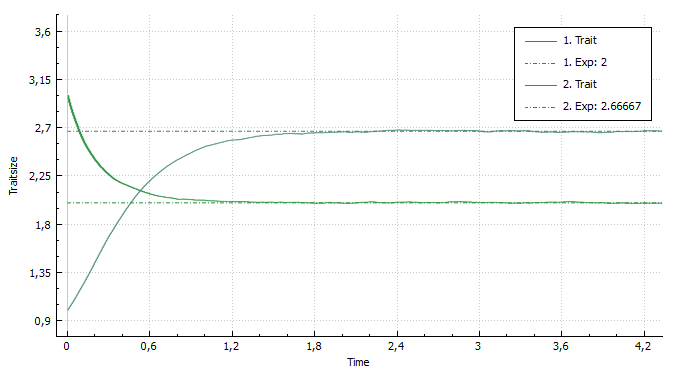
\includegraphics[width=1\linewidth]{./Pictures/BigKInstance_Equillibrium}
			\caption[Konvergenz_K=100000]{Konvergenz mit K=100000 und $ 15\cdot10^6 $ Sprüngen}
			\label{Konvergenz_K=100000}
		\end{figure}
	
	\subsection{Der TSS-Grenzwertprozess}
	Wie zuvor bei der LPA-Normalisierung erhalten wir TSS-Prozesse (Trait Substitution Sequence) als Grenzprozesse von BPDL-Prozessen mit großen Populationen und seltenen Mutationen. Mit wachsendem K  soll für die Mutationswahrscheinlichkeit durch die Vorschrift
	\begin{align}
		\frac{1}{e^{cK}} \ll \mu_K \ll \frac{1}{K \log(K)}, \qquad \forall c > 0, \label{TSSMutation}
	\end{align}
%	\[  \frac{1}{e^{cK}} \ll \mu_K \ll \frac{1}{K log(K)}, \qquad \forall c > 0,  \] 
	eine schnellere Konvergenz gegen 0 stattfinden, als die Geburten pro fester Zeiteinheit gegen unendlich streben. D.h. mit wachsendem K werden Mutationen zunehmend seltener.\\ 
	Der TSS-Prozess ist ein besonders interessanter Grenzprozess des BPDL-Prozesses, weil es ihm möglich ist, von einer monomorphen Population im Merkmal $ x $ zu einer anderen monomorphen Population mit Merkmal $ y $ zu springen, falls $ f(y,x) > 0 $ und $ f(x,y) < 0 $ (mehr dazu in Kapitel 7).\\
	In diesem Fall haben wir zu jeder festen Zeit höchstens zwei konkurrierende Merkmale. Diese Eigenschaft vereinfacht die Analyse des Prozesses sehr und ist der Wahl von $ \mu_K $ zu verdanken.\\
	\begin{figure}[H]
		\centering
		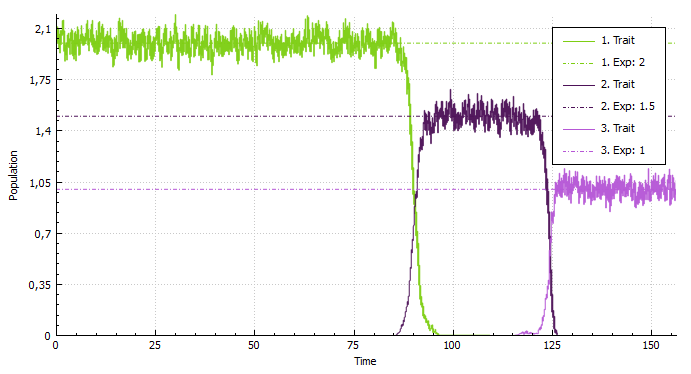
\includegraphics[width=0.8\linewidth]{../BachelorArbeit/Pictures/TSS2_pure_small}
		\caption[TSS-Prozess wechselnder Dominanz]{TSS-Prozess mit: K = 1000 und $ 4 \cdot 10^6 $ Sprüngen}
		\label{TSS_mitBPDLSimulator}
	\end{figure}
	\textbf{Frage:} Warum bietet $ \mu_K $ im Bereich (\ref{TSSMutation}) diese Eigenschaften?\\
	
	\textbf{Antwort:} Dank Freidlin und Wenzell \cite{freidlin2012random} erwarten wir, dass unsere dominante Spezies eine Zeit von der Ordnung $ \exp(cK) $ im Gleichgewicht bleibt. Schließlich können wir so kontrollieren, wie lange eine dominante Spezies, die für eine mutative Geburt in Frage kommt, erhalten bleibt. Dadurch, dass die Mutationen exponentiell verteilt sind, benötigt man eine Rate $ \mu_K \gg \frac{1}{e^{cK}} $ um eine Zeit von $ \exp(cK) $ nicht zu überschreiten, was die \textit{untere Schranke} rechtfertigt.\\
	Um die \textit{obere Schranke} zu rechtfertigen, betrachten wir nun die Zeit, die ein Mutant braucht, um ein dominantes Merkmal aussterben zu lassen. Das wird uns die Möglichkeit geben, einer neuen Mutation genug Zeit zu lassen bis das derzeit benachteiligte Merkmal ausgestorben ist.\\
	Angenommen es ereignet sich eine Mutation und der Mutant in $ y $ ist fitter ($ f(y,x) > 0, f(x,y) < 0 $), so wird mit positiver Wahrscheinlichkeit eine Invasion (näheres dazu im Kapitel 7 - TSS-Prozesse) ausgelöst. Wenn man Branching-Prozesse mit dem Lotka-Volterra-System vergleicht, kommt man darauf, dass die benötigte Zeit zum Verdrängen und Aussterben des ursprünglich dominanten Merkmals von der Ordnung $ \log(K) $ ist.
%	Diese Invasion wird eine Zeit von der Ordnung $ \log(K) $ benötigen. Das lässt sich folgern in dem man Branching Prozesse mit 
%	
	Skaliert man nun noch zusätzlich die Zeit, so führt dies dazu, dass der Prozess ausreichend Zeit zwischen zwei Mutationen hat, um ein benachteiligtes Merkmal zu verdrängen.
	Somit erlaubt uns die LPA-Annahme von einer deterministischen Populationsdynamik zwischen zwei Mutationen auszugehen \cite{raey}.\\
	
	
\section{Simulation}
In diesem Kapitel wird der Kern der Simulation algorithmisch näher untersucht. Dieser Kern besteht im Wesentlichen aus einem Sprung des BPDL-Prozesses.
Dabei wird zwischen der Implementierung und dem Pseudocode unterschieden, weil bei der Implementierung sorgfältig auf die Trennung der Aufgabenbereiche geachtet wurde, welche später beim Verhaltenstest sehr wichtig und im 5. Kapitel weiter verwendet werden.\\
Die hier verwendete Vorgehensweise unterscheidet sich von der aus \cite{fournier2004microscopic}, weil wir ein System mit vielen Individuen und wenigen Merkmalen betrachten, was uns ermöglicht, die individuellen Raten zu berücksichtigen.
	\subsection{Implementierung}
	Die Simulation durchläuft mehrere Schritte bis ein vollständiger Sprung von $ \nu_t $ abgeschlossen ist. Hier wird beschrieben in welcher Reihenfolge welche Schritte durchlaufen werden und welche Aufgabe diese erfüllen. Am Ende werden alle Funktionsaufrufe (Schritte) und Zusammenhänge in Abbildung \ref{fig:PseudoCodeForBThesis} als ein Ablauf-Tiefen-Diagramm illustriert.\\
	Im Code wird dabei objektorientiert mit Klassen und Objekten gearbeitet. Da diese Details nicht besonders von Interesse sind, wird eher ein heuristischer Überblick der Implementierung gegeben. So kann hier z.B. angenommen werden, dass die Variable "{}Members[i]"{} Zugriff auf die Anzahl der Individuen des i-ten Merkmals bietet, was im Code jedoch komplexer realisiert werden musste.\\
	
	\subsubsection{Raten berechnen}	
	Bevor ein Merkmal und Ereignis ausgewählt werden kann, müssen die Raten bekannt sein, nach denen die exponentiellen Uhren gestellt werden.\\
	Die Todesrate setzt sich aus der intrinsischen Todesrate und der durch Wettbewerb zusammen und ist zu Beginn 0.\\
	
	Die folgende Funktion addiert die intrinsische Todesrate zur aktuellen Todesrate. Dabei wird direkt das Superpositionsprinzip genutzt, um die gesamte intrinsische Todesrate des Merkmals in "{}TotalDeathRate[i]"{} aufzuaddieren.
	\begin{algorithm}[H]
		\caption{addTotalIntrinsicDeathRateOf(TraitIndex: i)}
		\begin{algorithmic}[1]
			\Ensure{addiert zur Todesrate die intrinsische-Todesrate}
			\State TotalDeathRate[i] = DeathRate[i] $ \cdot $ Members[i]
		\end{algorithmic}
	\end{algorithm}
	Diese Funktion addiert die wettbewerbliche Todesrate zur aktuellen Todesrate.
	\begin{algorithm}[H]
		\caption{addTotalCompDeathRateOf(TraitIndex: i)}
		\begin{algorithmic}[1]
			\Ensure{addiert zur Todesrate die Wettbewerbs-Todesrate}
			\For{j=0 $ \to $ n-1}
				\State TotalDeathRate[i] += CompDeathRate[i,j] $ \cdot $ Members[i] $ \cdot $ Members[j];
			\EndFor
		\end{algorithmic}
	\end{algorithm}
	Die auf den ersten Blick übertrieben erscheinende Trennung der beiden Funktionen ist für das verwendete Programmierkonzept entscheidend, nach dem jeder Funktion eine möglichst eindeutige Aufgabe zukommen soll \cite{martin2008clean}. Darauf wird näher im nächsten Kapitel eingegangen. \\
	Schließlich erfolgt aus obigem die Berechnung der Totalen Todesraten:
	\begin{algorithm}[H]
		\caption{calculateTotalDeathRates()}
		\begin{algorithmic}[1]
			\Ensure{berechnet die gesamten Todesraten aller Merkmale}
			\For{i=0 $ \to $ n-1}
				\State TotalDeathRate[i] = 0;
				\State addTotalIntrinsicDeathRateOf(i);
				\State addTotalCompDeathRateOf(i);
			\EndFor
		\end{algorithmic}
	\end{algorithm}
	Danach kommen wir zur Berechnung der Geburtsrate pro Merkmal. Auch hier sollten Mutationen und intrinsische Geburten gesondert berechnet werden. Zusammengefasst:
	\begin{algorithm}[H]
		\caption{calculateTotalBirthRates()}
		\begin{algorithmic}[1]
			\Ensure{berechnet die gesamten Geburtsraten aller Merkmale}
			\State $ \qquad $ $ \downarrow $ \textbf{intrinsische Geburtenrate} $ \downarrow $
			\For{i=0 $ \to $ n-1}
				\State TotalBirthRate[i] = Members[i] $ \cdot $ BirthRate[i] $ \cdot $ (1 - Mutation);
			\EndFor
			\State $ \qquad $ $ \downarrow $ \textbf{Mutationsraten} $ \downarrow $
			\For{i=1 $ \to $ n-2}
				\State TotalBirthRate[i] += Members[i-1] $ \cdot $ BirthRate[i-1] $ \cdot $ Mutation $ \cdot $ 0.5;
				\State TotalBirthRate[i] += Members[i+1] $ \cdot $ BirthRate[i+1] $ \cdot $ Mutation $ \cdot $ 0.5;
			\EndFor
			\State TotalBirthRate[0] += Members[1] $ \cdot $ BirthRate[1] $ \cdot $ Mutation $ \cdot $ 0.5;
			\State TotalBirthRate[n-1] += Members[n-2] $ \cdot $ BirthRate[n-2] $ \cdot $ Mutation $ \cdot $ 0.5;
		\end{algorithmic}
	\end{algorithm}
	 Jetzt sind wir bereit eine Funktion aufzurufen, die aus den vorher berechneten Geburts- und Todesraten pro Merkmal durch Superposition eine totale Eventrate berechnet, nach der wir eine exponentielle Uhr stellen können, die schließlich das Klingeln der ersten aller Merkmalsuhren simuliert.
	 \begin{algorithm}[H]
 		\caption{calculateTotalEventRate()}
 		\begin{algorithmic}[1]
 			\Ensure{berechnet die totale Ereignisrate}
 			\State TotalEventRate = 0;
 			\For{i=0 $ \to $ n-1}
 				\State TotalTraitRate[i] = TotalBirthRate[i] + TotalDeathRate[i];
 				\State TotalEventRate += TotalTraitRate[i];
 			\EndFor
 		\end{algorithmic}
 	\end{algorithm}
 	Hier fällt auf, dass wir auch die \textit{TotalTraitRate} oder Totale Merkmalsrate gespeichert haben. Diese repräsentiert die gesamte Ereignisrate eines Merkmals.\\
 	Zum Schluss sollte es eine Funktion geben, die alle bisherigen Funktionen in der richtigen Reihenfolge ausführt und so die Berechnung aller Ereignisraten sichert:
 	\begin{algorithm}[H]
 		\caption{calculateEventRates()}
 		\begin{algorithmic}[1]
 			\Ensure{stellt sicher, dass alle akutellen Raten berechnet wurden}
 			\State calculateTotalDeathRates();
 			\State calculateTotalBirthRates();
 			\State calculateTotalEventRate();
 		\end{algorithmic}
 	\end{algorithm}
	
	\subsubsection{Ereignis und Zeit bestimmen}
	
	Mit den zuvor berechneten Raten ist es einfach, die Dauer bis zum nächsten Ereignis zu bestimmen. An dieser Stelle verwende ich die Funktion \textit{rollExpDist(Parameter)} zum Ziehen einer exponentiell verteilten Zufallsvariable, die nicht weiter interessant ist und deshalb nicht erläutert wird.
 	\begin{algorithm}[H]
 		\caption{sampleEventTime()}
 		\begin{algorithmic}[1]
 			\Ensure{Zieht die nächste Ereigniszeit}
 			\State EventTime = rollExpDist(TotalEventRate);
 			\State Timeline += EventTime;
 		\end{algorithmic}
 	\end{algorithm}
 	Jetzt bleibt zu bestimmen, wem was passiert, also welches Ereignis welches Merkmal treffen wird. Dafür wenden wir das Superpositionsprinzip in anderer Richtung an als bisher:\\
 	Zum Bestimmen des auserwählten Merkmals beachten wir den Anteil der Merkmale an der Totalen Eventrate. Dieser ist klar erkennbar durch die Summe:
 	\[ \text{TotalTraitRate} = \sum_{i = 0}^{n - 1} \text{TotalTraitRate[i]} \]
 	Also hat das $ i\text{-}te $ Merkmal mit Wahrscheinlichkeit $ \frac{TotalTraitRate[i]}{TotalEventRate} $ das Ereignis ausgelöst. Um also das verantwortliche Merkmal auszuwählen, können wir eine uniform verteilte Zufallsvariable ziehen und entscheiden, welche der Merkmalsraten damit gemeint ist. Abbildung \ref{SelectTrait} illustriert den Auswahlprozess.
 	\begin{figure}[H]
		\centering
		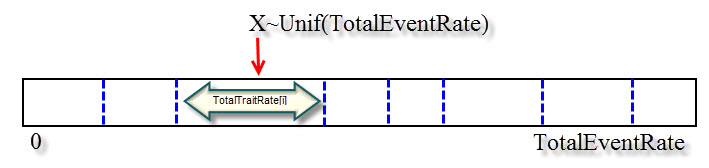
\includegraphics[width=1\linewidth]{./Pictures/SelectTrait}
		\caption[]{Auswahl des Merkmals nach Anteil an der TotalEventRate}
		\label{SelectTrait}
	\end{figure}
	Im Code wird dafür iterativ geprüft, ob "{}X $ \sim $ Unif(TotalEventRate)"{} im ersten Intervall der Länge TotalTraitRate[0] liegt. 
	\begin{itemize}
		\item[] Falls ja, so wird dieses Merkmal gewählt und die Funktion wird verlassen.
		\item[] Falls nicht, so wird das Merkmal $ 0 $ aus den relevanten Merkmalen entfernt und X wird um die Intervallänge TotalTraitRate[0] reduziert, um schließlich erneut mit dem ersten relevanten Intervall verglichen zu werden (jetzt TotalTraitRate[1]). Auf diese Weise nähert man sich immer weiter dem getroffenen Merkmal:
	\end{itemize}
	\begin{algorithm}[H]
 		\caption{choseTraitToChange()}
 		\begin{algorithmic}[1]
 			\Ensure{wählt ein Merkmal zum Ändern aus}
 			\State X = rollUnifDist(TotalEventRate);
 			\For{i=0 $ \to $ n-1}
 				\If{X $ \le $ TotalTraitRate[i]}
 					\State ChosenTrait = i;
 					\State return;
 				\EndIf
 				\State X -= TotalTraitRate[i];
 			\EndFor
 		\end{algorithmic}
 	\end{algorithm}
 	Auf dieselbe Weise wird entschieden, welches Ereignis eintrifft und anschließend in \textit{isBirth} gespeichert. Da wir hier jedoch nur Geburt und Tod zur Auswahl haben, würde sich natürlich eine Bernoulli verteilte Zufallsvariable ergeben mit:
 	\[ \text{isBirth} \sim \text{Ber(TotalBirthRate[ChosenTrait])} \]
 	Im Code wurde \textit{isBirth} folgendermaßen gezogen:
	\begin{algorithm}[H]
 		\caption{choseEventType()}
 		\begin{algorithmic}[1]
 			\Ensure{wählt ein Ereignis für das entsprechende Merkmal aus}
 			\State X = rollUnifDist(TotalTraitRate[ChosenTrait]);
 			\If{X $ \le $ TotalBirthRate[ChosenTrait]}
 				\State isBirth = true;
 			\Else
 				\State isBirth = false;
 			\EndIf
 		\end{algorithmic}
 	\end{algorithm}
 	Danach muss noch das Ereignis aus Alg. 9 auf das Merkmal aus Alg. 8 angewendet werden.
	\begin{algorithm}[H]
 		\caption{executeEventTypeOnTrait()}
 		\begin{algorithmic}[1]
 			\Ensure{wendet das gewählte Ereignis auf das gewählte Merkmal an}
 			\State X = rollUnifDist(TotalTraitRate[ChosenTrait]);
 			\If{isBirth}
 				\State Members[ChosenTrait] += 1;
 			\EndIf
 			\If{$ \neg \text{isBirth} $ \& Members[ChosenTrait] $ > $ 0}
 				\State Members[ChosenTrait] -= 1;
 			\EndIf
 		\end{algorithmic}
 	\end{algorithm} 	
 	Zum Schluss wird noch eine Funktion erstellt, welche das Ausführen eines Ereignisses in richtiger Reihenfolge realisiert und in einem Schritt aus gegebenen Raten die Veränderung der Population durchführt.
 	\begin{algorithm}[H]
 		\caption{changeATrait()}
 		\begin{algorithmic}[1]
 			\Ensure{lässt ein Ereignis ein Merkmal treffen}
 			\State choseTraitToChange();
 			\State choseEventType();
 			\State executeEventTypeOnTrait();
 		\end{algorithmic}
 	\end{algorithm} 
	Aus diesen 3 wesentlichen Schritten
	\begin{itemize}
		\item Raten berechnen
		\item Ereigniszeit ziehen
		\item Ereignis eintreten lassen
	\end{itemize}
	kann schließlich eine sehr übersichtliche Funktion konstruiert werden, die einen kompletten Sprung des Prozesses durchführt.
	\begin{algorithm}[H]
 		\caption{makeEvolutionStep()}
 		\begin{algorithmic}[1]
 			\Ensure{lässt ein Ereignis ein Merkmal treffen}
 			\State calculateEventRates();
 			\State sampleEventTime();
 			\State changeATrait();
 		\end{algorithmic}
 	\end{algorithm}
	 	
	\subsubsection{Übersicht}
	Hier ist eine Übersicht aller Funktionen, ihrer Reihenfolge und Aufruftiefe. \\
	Die Funktionen wurden auf Englisch beschrieben, weil sie damit eine Referenz zu der im Quellcode beschriebenen Funktion darstellen. Z.B. "{}make one evolution step"{} verweist auf die Funktion "{}makeEvoultionStep"{}, oder "{}calculate event rates"{} $ \to $ "{}calculateEventRates"{} etc.
	\begin{figure}[H]
		\centering
		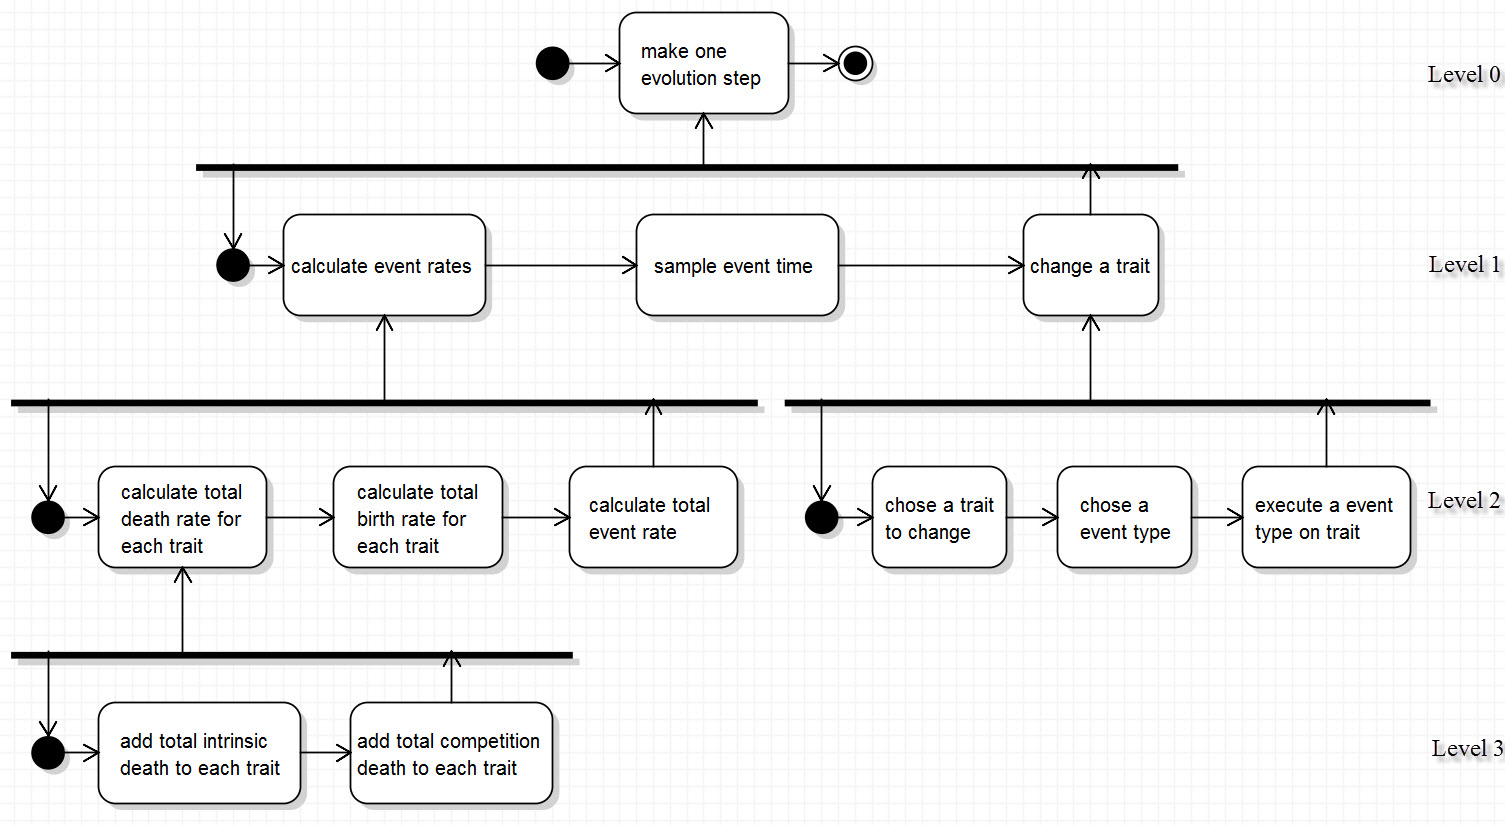
\includegraphics[width=1\linewidth]{../UMLs/PseudoCodeForBThesis}
		\caption{Diagramm mit Funktionsaufrufen und ihren Tiefenebenen}
		\label{fig:PseudoCodeForBThesis}
	\end{figure}
	
	\subsection{Pseudocode}
	Natürlich lässt sich der Ablauf eines Sprunges auch durch Pseudocode in eine Funktion "{}makeEvoultionStep"{} zusammenfassen.\\
	Im Pseudocode finden sich in blau einige Verweise auf die zuvor beschriebene Implementierung.
	
	\begin{algorithm}[H]
		\caption{makeEvolutionStep() - Part 1}
		\begin{algorithmic}[1]
			\Ensure{A full evolution Step happened}
			\Require $ t, X = \{0,\dots, n-1\} $
			\For{ $ x \in X $ }\Comment{$ \downarrow $ \textcolor[rgb]{0,0,0.55}{calculateEventRates}() $ \downarrow $}
				\State $  D(x) := n_t(x) \cdot \left( d(x) + \sum_{y \in X} c(x,y) \cdot n_t(y) \right) $
				\State $ B(x) := \underbrace{b(x) \cdot (1 - \mu) \cdot n_t(x)}_{arteigene}  $
				\If{$ x > 0 $}
					\State $ B(x) += \underbrace{b(x-1)\cdot n_t(x-1)}_{Mutation Links} \cdot \frac{\mu}{2} $
				\EndIf
				\If{$ x < n-1 $}
					\State $ B(x) += \underbrace{b(x+1)\cdot n_t(x+1)}_{Mutation Rechts} \cdot \frac{\mu}{2} $
				\EndIf
				\State $ TotalTraitRate(x) = B(x) + D(x) $
			\EndFor
			\State $ TotalEventRate := \sum_{x \in X} TotalTraitRate(x) $
			\State sample $ Z \sim exp(TotalEventRate) $ \Comment{$\downarrow $ \textcolor[rgb]{0,0,0.55}{sampleEventTime}() $ \downarrow $} 
			\State $ t += Z $
			
			\State sample $ Y \sim U(0,TotalEventRate) $ \Comment{$ \downarrow $ \textcolor[rgb]{0,0,0.55}{choseTraitToChange}() $ \downarrow $}
			\For{$ x \in X $}
				\If{$ Y \le TotalTraitRate(x) $}
					\State $ ChosenTrait := x $
					\State break
				\EndIf
				\State $ Y -= TotalTraitRate(x) $
			\EndFor 
			
			\State sample $ Y \sim U(0,TotalTraitRate(ChosenTrait)) $
			\If{$ Y \le B(ChosenTrait) $} \Comment{$ \downarrow $ \textcolor[rgb]{0,0,0.55}{choseEventType()} $ \downarrow $}
				\State isBirht := true
			\Else
				\State isBirth := false
			\EndIf
			\If{isBirth} \Comment{$ \downarrow $
				\textcolor[rgb]{0,0,0.55}{executeEventTypeOnTrait()} $ \downarrow $}
				\State $ n_t(ChosenTrait) += 1 $
			\Else
				\If{$ n_t(ChosenTrait) \ge 0 $}
					\State $ n_t(ChosenTrait) -= 1 $
				\EndIf
			\EndIf
		\end{algorithmic}
	\end{algorithm}
	
	\subsection{Optimierung für viele Merkmale}
	Für eine Simulation ist klar, dass in Abhängigkeit der Sprünge (ggf. hoher) linearer Aufwand zu erwarten ist. Zwar ist dieser am Modell nachvollziehbar, jedoch konnte wegen der Wettbewerbsrate ein quadratischer Aufwand in der Anzahl der Merkmale nicht vermieden werden. Die diesbezüglich von mir vorgenommene Optimierung ist bereits ab dem ersten Merkmal von Nutzen (praktisch wurde dieser jedoch erst ab dem 2. gemessen, vgl. Abb. \ref{Test Results})), und somit trotz der stets überschaubaren Menge an Merkmalen in unserer Simulation relevant.\\
	Nach meinen Tests, die später im Kapitel "{}Verhaltenstest"{} eingeführt werden, ergab sich, wie zu erwarten, der größte zeitliche Aufwand in der Berechnung der Raten (genauer: der Todesraten). Die Optimierung vermeidet die komplette Neuberechnung der Raten, sondern führt stattdessen zu deren Anpassung.\\
	Dazu werden die Raten nicht zu Beginn berechnet, wie zuvor in Algorithmus 12 "{}makeEvolutionStep()"{} in der 1. Zeile. Stattdessen wird mit den aktuellen Raten eine Ereigniszeit gezogen "{}sampleEventTime()"{} und anschließend ein Ereignis ausgelöst "{}changeATrait()"{}, welches es ermöglicht die nächsten Raten anzupassen "{}adjustNewEventRates()"{}. Dafür wird zunächst unterschieden, ob ein Tod oder eine Geburt eingetreten ist. Das lässt sich leicht mit der in Algorithmus 9 erwähnten "{}isBirth"{} Variable entscheiden.\\
	Angenommen es ereignet sich eine Geburt. Damit können zusammen mit dem ausgewählten Merkmal "{}chosenTrait"{} folgende Anpassungen gemacht werden:
	\begin{itemize}
		\item Die \textbf{intrinsische Todesrate} von "{}chosenTrait"{} wird um  die des geborenen Individuums erhöht:\\ 
		TotalDeathRate[chosenTrait] += DeathRate[chosenTrait];
		\item Die \textbf{Todesrate durch Wettbewerb} wird bei jedem Merkmal um das geborene Individuum erhöht:\\
		TotalDeathRate[i] += CompDeathRate[i][chosenTrait]; $ \qquad \forall \text{ i} \in X $
		\item Die \textbf{Geburtsraten} werden genauso wie die Todesraten behandelt:\\
		TotalBirthRate[chosenTrait] += BirthRate[chosenTrait];
		\item Entsprechend auch die \textbf{Mutationsraten}:\\
		TotalBirthRate[i] += Mutation $ \cdot $ 0.5 $ \cdot $ BirthRate[chosenTrait]; \\
		$\forall \text{ i } \sim \text{ chosenTrait} $
		\item Zum Schluss noch die \textbf{Totale Ereignisrate}:\\
		Eine erneute Berechnung aller Totalen Raten kann hier nicht vermieden werden.
	\end{itemize}
	Man erkennt, dass hier keine quadratische Abhängigkeit der Merkmale mehr zu finden ist.
	
	\subsection{Normalisierung}
	Weder in der Implementierung noch im Pseudocode war bisher von Normalisierung die Rede. Dies liegt darin begründet, dass sie vom Programmkern getrennt wurde, da sie den wesentlichen evolutionären Mechanismus nicht beeinflusst, sondern nur die Sichtweise darauf verändert.\\
	Um diese Trennung zu realisieren wurde an zwei Stellen Veränderungen vorgenommen.
	\begin{itemize}
		\item [\textbf{1.}] Unmittelbar nach dem Einlesen der Parameter wurde sowohl die Wettbewerbsrate durch K geteilt als auch die Startpopulation um K hoch skaliert. Auf diese Weise kann der Programmkern ohne Kenntnis eines K die Evolution durchführen.\\ 
		Dadurch lässt sich ein Prozess ohne Rücksicht auf anzupassende Parameter durch wachsendes K verfeinern, sodass die Konvergenz mit wachsendem K wie in Abbildung \ref{Konvergenz_K=100000} verfolgt werden kann.
		\item [\textbf{2.}] Trotz der Berechnung der Ergebnisse ohne Rücksicht auf ein vorhandenes K sollte die Darstellung natürlich reskaliert erfolgen ($ \nu_t^K = \frac{\nu_t}{K} $). Deswegen ist es außerhalb des Programmkerns nur über einen sogenannten "{}getter"{} (eine spezielle Zugriffsfunktion) möglich auf die Mitglieder eines Merkmals zuzugreifen. Dieser "{}getter"{} liefert stets den reskalierten Wert zurück.\\
	\end{itemize}
	
	\subsubsection{Sehr viele Sprünge}
	Gerade bei der Normalisierung wird es mit wachsendem K notwendig, besonders viele Sprünge zu machen. Die Anzahl der Sprünge übersteigt schnell das Fassungsvermögen eines Arrays.	Um auch mehr als 100 Millionen Punkte speichern zu können, wurden zwei Lösungen implementiert:\\
	\begin{itemize}
		\item[\textbf{1.}] Die "{}erweiterten Sprünge"{} sind eine Lösung, die zur Zeit angewendet wird. Zu Beginn der Simulation wird anhand der maximalen Iterationen entschieden wie viel Speicher benötigt wird und eine "{}Jumps"{}-Variable gesetzt. Diese "{}Jumps"{} Variable enthält die Anzahl der Spr\-ünge bis ein Punkt gespeichert wird. So wird bei 100 Millionen Iterationen nur jeder zehnte Punkte gespeichert. \\
		\item[\textbf{2.}] Eine weitere Lösung ist die "{}storePoint()"{} Funktion. Sie erstellt zu Beginn der Rechnung eine Datei und hängt immer weiter Punkte an bis die Berechnung vorbei ist.\\
		Schließlich wird die Graphklasse einzeln jeden Punkt an den Graphen anhängen.\\ 
		Diese Variante ist implementiert und wurde getestet. Sie ist auch in einem Unit Test enthalten, der aber nicht in Kapitel 6 erläutert wird.
	\end{itemize}

	
\section{Das Programm}
In diesem Kapitel werden die Programme und ihre Entwicklung vorgestellt. Dabei wird darauf eingegangen, welche Möglichkeiten es gibt eine GUI zu entwickeln, welche Architektur und welcher Codestil im Programm verwendet wurden, wie das Layout gewählt wurde und wie das Programm zu bedienen ist.\\
Zunächst sei gesagt, dass die Programme zum Zeitpunkt der Erstellung der Bachelorarbeit noch nicht völlig fertig gestellt sind. Es gibt noch überflüssige Funktionen im TSS-Simulator und noch einige Wünsche zur erweiterten Verwendung des Programms. 

	\subsection{GUI - Entwicklung}
	Ziel war es, ein Programm mit einer graphischen Oberfläche in C++ zu schreiben. Nach \cite[14 - Grafische Benutzungsschnittstellen]{breymann2011c++} kennt Standard C++ keine Elemente für grafische Benutzungsoberflächen (englisch \textit{graphical user interfaces - GUI}). Weil in unserem Fall aber nicht auf eine solche verzichtet werden konnte, wird hier kurz vorgestellt, welche Varianten der GUI-Programmierung es gibt und wie unsere Auswahl begründet ist.\\
	
	\textbf{MFC}\\
	Sehr bekannt sind die Microsoft Foundation Classes (MFC) bzw. ihre Nachfolger in .NET für Windows Betriebssysteme. Aber genau hier liegt bereits das Problem. In unserem Fall wurden die Programme für zwei Mitarbeiter entwickelt, welche jeweils MAC verwendeten, an einem Institut, welches überwiegend mit Ubuntu arbeitet. Deswegen kam MFC nicht in Frage.\\
	
	\textbf{$ \text{GTK}_+ $ }(the GIMP Toolkit)\\
	$ \text{GTK}_+ $ ist eine weitere Bibliothek zur Erstellung von GUI's. Sie wurde haupt\-sächlich für das Bildbearbeitungsprogramm GIMP, entwickelt. $ \text{GTK}_+ $ wird zur Entwicklung des GNOME-Desktops benutzt, welche auf vielen Linux Systemen zu finden sind. Aber auch dazu gibt es eine bessere Alternative.\\
	
	\textbf{Qt}\\
	Die portable Qt-Bibliothek ist sehr bekannt und lässt sich sehr einfach auf Windows-, Mac- und Unix-Betriebssysteme portieren. Die aus manchen Linux-Systemen bekannte Benutzungsoberfläche KDE wird mit Qt entwickelt. Damit bietet sich Qt bereits jetzt als eine gute Option zur Entwicklung für alle Betriebssysteme an.\\
	Hinzu kommen noch viele weitere Vorteile, wie die große Auswahl an Hilfsprogrammen und Bibliotheken, die sehr ausführliche Dokumentation , und dass es sich um eine Open Source Software handelt.\\
	"{}Zusammengefasst: Qt ist die ausgereifteste und umfangreichste Open Source Software für die portable Entwicklung grafischer Benutzungsoberflächen mit C++"{}\cite[S.452]{breymann2011c++}.

	\subsection{Architektur und Module}
	Zuerst möchte ich die grobe Architektur des Programmcodes vorstellen. Diese kann in drei Module zusammengefasst werden, welche möglichst wenige Schnittstellen untereinander verwenden und damit viel Unabhängigkeit bieten.
	
	\begin{itemize}
		\item [\textbf{1.}] "{}Population Kernel"{}\\
		Der Programmkern besteht aus dem "{}Population Kernel"{}, welcher ausschließlich für die Berechnungen zuständig ist. Hier werden keine historischen Daten gespeichert, womit dieser Bereich immer nur die Daten der Population zur aktuellen Berechnung bereit hält. Also enthält dieser nur eine Sammlung von Funktionen, die das Modell befragen können.\\
		Die einzige Klasse dieses Moduls, mit der eine Kommunikation nach außen möglich ist, ist der "{}TraitEventManager"{}, der, wie der Name schon sagt, die Ereignisse und Merkmale verwaltet (Abb. \ref{Module und Klassen}, rechts).\\
		Das Besondere am "{}Population Kernel"{} ist, dass er mit Standard C++11 implementiert wurde und somit überall wiederverwendbar ist. Er ist leicht zu verändern und sehr flexibel, weshalb man unseren Kern z.B. durch einen anderen ersetzten könnte, ohne Anpassungen an anderen Modulen vornehmen zu müssen. So kann man die simulierten Modelle variieren, solange jedes Modell in der Lage ist, einen unabhängigen Sprung durchzuführen.\\
		\item [\textbf{2.}] "{}Graph Management"{}\\
		Der zweite Bereich organisiert alle Daten, die die Simulation anfragen kann. Hier liegen der eigentliche Speicher und die Kommunikation zwischen GUI und Algorithmus.\\
		Es ist eine Art Hilfsklasse, die eine Kommunikation zwischen den Modulen ermöglicht. Zu diesem Zweck wurde hier bereits die Qt-Bibliothek verwendet, um Daten für die GUI abholbereit anzubieten.\\
		Sie erhält die Wünsche des Users in Form von Anweisungen aus der "{}GUI"{} und verwendet die Möglichkeiten des "{}Population Kernel"{}, um entsprechende Daten abrufbereit zu erstellen.
		\item [\textbf{3.}] "{}GUI"{}\\
		Das letzte und unflexibelste Modul umfasst die grafische Benutzungsoberfläche. Hier kommen zwei wichtige Klassen zum Einsatz.\\
		Die erste, "{}MainWindow"{}, ist das Hauptfenster, in dem der Nutzer die Parameter festlegen und, wenn alles stimmt, auch die Simulation starten kann. Für eine möglichst große Übersicht bei der Analyse der Ergebnisse, verwendet das Hauptfenster eine weitere Klasse, "{}PlotWindow"{}, welche ein extra Fenster mit Graphen öffnet (Plot-Fenster).\\
		Wie man vermuten kann, wird hier bereits etwas zum Darstellen eines Graphen, also fast ausschließlich Qt-Programmierung verwendet.\\
		Dieses Plot-Fenster verwendet ein "{}GraphClass"{}-Objekt, um einen Graphen erstellen zu können. Natürlich ist es für die Verwendung der Daten selbst verantwortlich.
	\end{itemize}	
 	
 	Die folgende Abbildung \ref{Module und Klassen} stellt zusammenfassend die obigen Module und die Klassenhierarchie dar:
	\begin{figure}[H]
		\centering
		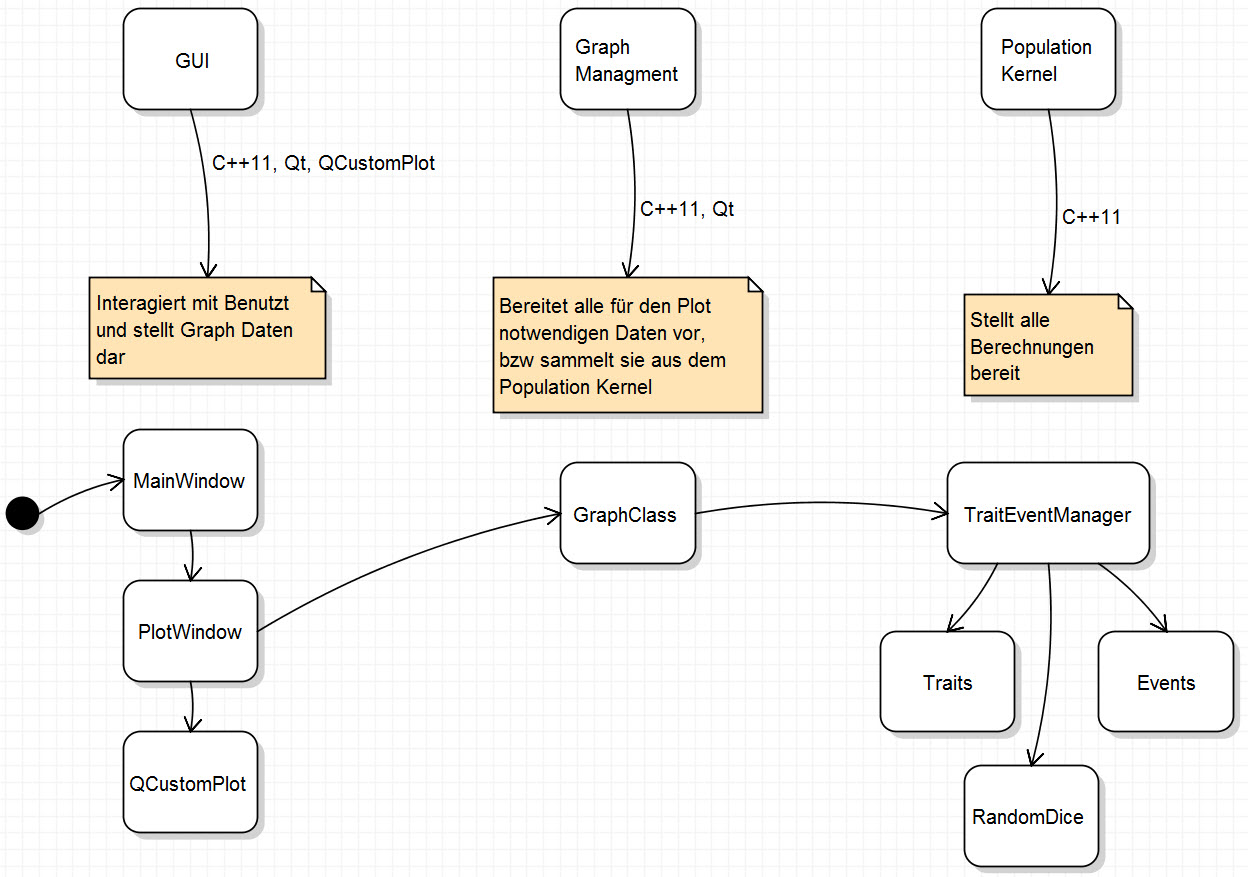
\includegraphics[width=1 \linewidth]{./Pictures/Bild_Module}
		\caption[Module]{Arbeitsmodule und Klassenabhängigkeiten}
		\label{Module und Klassen}
	\end{figure}	
		
	\subsection{Flexibilität und agile Softwareentwicklung}
	Die Idee der getrennten Aufgabenbereiche geht darauf zurück, dass eine möglichst große Unabhängigkeit zwischen Arbeitsschritten notwendig ist, um das Programm flexibel zu halten und sogenannten "{}Coderot/Software\-erosion"{} (faulen Code) zu verhindern \cite{martin2008clean}. Dieser bezeichnet die zunehmende Entropie einer Software. Das heißt sie führt mit zunehmender Weiterentwicklung der Software zu einer Verringerung der Leistung, Erschwernissen bei der Anpassbarkeit bzw. Flexibilität und in zunehmendem Maße zu undefiniertem Verhalten.\\
	In der Softwareentwicklung ist undefiniertes Verhalten schwer zu behandeln, da man keine Fehler beim Compilieren oder Ausführen erhält. Es wird lediglich ein nicht nachvollziehbares Verhalten des Programms festgestellt, welches sich im obigen Falle nur noch sehr schwer im Code eingrenzen lässt.\\
	
	Außerdem wurde darauf geachtet, dass jede Klasse nur eine möglichst fest definierte Aufgabe zu erfüllen hat. In einer Klasse sollten lediglich Funktionen vorhanden sein, die zur Erfüllung dieser Aufgabe beitragen. Dieses Prinzip trägt den Namen "{}Single-Responsibility-Prinzip"{} und wurde von Robert C. Martin in \cite{Martin:2003:ASD:515230} eingeführt. Die dort beschriebene "{}Agile Softwareentwicklung"{} fand auch Anwendung bei der Neuorganisation von Zielen und Wünschen mit Loren Coquille und Martina Baar, wird aber hier nicht weiter erläutert.
	
	\subsection{Layout}
	Hier wird die Oberfläche des Programms vorgestellt.
	\subsubsection{Lesen und Anzeigen von Parametern}
	Die Bedienung des Programms sollte das Lesen und Anzeigen der Merkmals-Parameter bereitstellen. Da es viele Parameter gibt und die Anzahl der Parameter quadratisch mit der Anzahl der betrachteten Merkmale steigt, bietet sich das Lesen aus zuvor erstellten Dateien an.\\
	Dabei werden die Daten aus den Dateien in folgender Reihenfolge zeilenweise ausgelesen Abbildung \ref{Parameter}:
	\begin{itemize}
		\item $ m $: Anzahl der Merkmale
		\item $ K $: Parameter
		\item $ \mu $: Mutationswahrscheinlichkeit
		\item $ c(1,1) \text{ } \dots \text{ } c(1,m) $: 1. Zeile der Wettbewerbsraten \\
			$ \vdots $\\
			$ c(m,1) \text{ } \dots \text{ } c(m,m) $: m. te Zeile der Wettbewerbsraten 
		\item $ n_0(1) $: Populationsgröße des 1. Merkmals: \\
			$ \vdots $\\
			$ n_0(m) $: Populationsgröße des m. Merkmals: 
		\item $ b(1) $: Geburtenrate des 1. Merkmals\\
			$ \vdots $\\
			$ b(m) $: Geburtenrate des m. Merkmals
		\item $ d(1) $: Todesrate des 1. Merkmals\\
			$ \vdots $\\
			$ d(m) $: Todesrate des m. Merkmals
	\end{itemize}
	
	\begin{center}
	\begin{minipage}{0.15\textwidth}
		\begin{figure}[H]
			\centering
			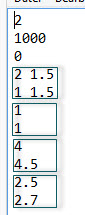
\includegraphics[width=1\linewidth]{./Pictures/Parameter}
			\caption[Parameter]{Datei}
			\label{Parameter}
		\end{figure}
	\end{minipage}
	$ \quad $
	\begin{minipage}{0.6\textwidth}
		Dabei wird $ \mu $ und $ c $ natürlich ohne Skalierung mit $ K $ angegeben. Die Gründe dafür wurden in Kapitel 4.4 beschrieben.\\
		
		Nebenstehend sieht man ein Beispiel einer Instanz mit zwei Merkmalen, $ K = 1000 $, $ \mu = 0 $ usw., wobei die Markierungen die Wettbewerbsmatrix, die Startpopulation, die Geburtenraten und die Todesraten enthalten.\\
	\end{minipage}
	\end{center}
	
	Das Programm muss also die Eingabe eines gültigen Dateinamens fordern, bevor eine Simulation gestartet werden kann. Deshalb werden bis zum Zeitpunkt gelesener Parameter alle nicht relevanten Schaltflächen deaktiviert und nur ausgegraut angezeigt Abbildung \ref{MainWindow_Start}, gelb markiert.\\
	Sobald man einen Namen in das einzig mögliche Feld eingegeben hat, kann man zwischen den Schaltflächen "{}load File"{} und "{}create File"{} wählen (Abbildung \ref{MainWindow_Start}, rot markiert).\\
	
	\begin{figure}[H]
		\centering
		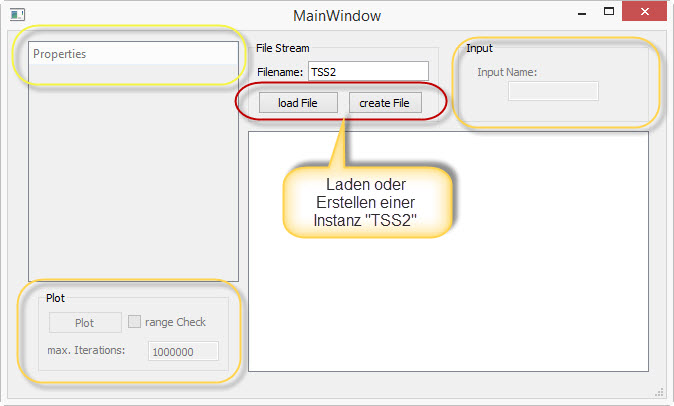
\includegraphics[width=1\linewidth]{./Pictures/MainWindow_Start}
		\caption[Startwindow]{MainWindow nach dem Start}
		\label{MainWindow_Start}
	\end{figure}
	Wie schon zuvor erwähnt, ist dem Programm vorab unbekannt, welchen Umfang die gelesenen Parameter haben werden, weshalb die Entscheidung der Darstellung auf eine Baumstruktur fiel.\\
	Sie hat bei der Initialisierung immer denselben Umfang (Abbildung \ref{Baumstruktur_geschlossen}) und der gewünschte Ast lässt sich einfach erweitern (Abbildung \ref{Baumstruktur_offen}).
	\begin{center}
	\begin{minipage}{0.45\textwidth}
		\begin{figure}[H]
			\centering
			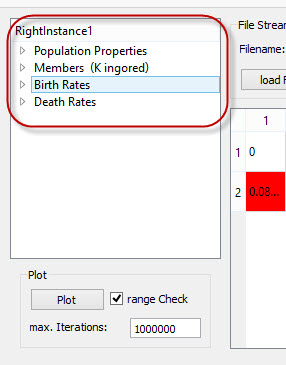
\includegraphics[width=1\linewidth]{./Pictures/MainWindow_ParameterBaum_zu}
			\caption[MainWindow_Parameter]{Baumstruktur - geschlossen}
			\label{Baumstruktur_geschlossen}
		\end{figure}
	\end{minipage} $ \quad $
	\begin{minipage}{0.45\textwidth}
		\begin{figure}[H]
			\centering
			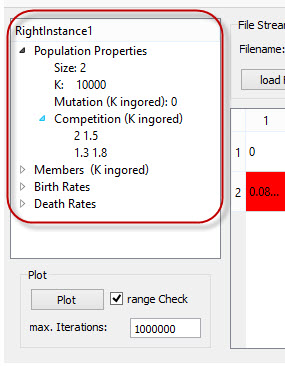
\includegraphics[width=1\linewidth]{./Pictures/MainWindow_ParameterBaum_offen}
			\caption[MainWindow_Parameter]{Verzweigte Baumstruktur - geöffnet}
			\label{Baumstruktur_offen}
		\end{figure}
	\end{minipage}
	\end{center}
		
	\subsubsection{Schreiben neuer Testinstanzen}
	Die letzte Herausforderung bestand darin, eine Instanz durch das Programm geleitet erstellen zu können. Während diese Aufgabe bei einer Konsolenanwendung (bekannt aus den klassischen C-Programmen) denkbar einfach mit "{}printf"{} und "{}scanf"{} erledigt werden konnten, stößt man hier auf das Problem der sogenannten "{}Ereignisgesteuerten Programmierung"{} \cite{breymann2011c++}.\\
	Während zuvor die Reihenfolge der Programmschritte vorbestimmt war, so gilt das nicht mehr für graphische Benutzungsoberflächen. In unserem Fall ist die Reihenfolge der Interaktionsschritte eines Benutzers, z.B. Anklicken oder Mausbewegung, nicht vorhersehbar und damit auch nicht die Reihenfolge der auszuführenden Programmschritte.\\
	Es geht also darum, Funktionen zu schreiben, die nicht an anderer Stelle vom Programm, sondern bei Eintreffen eines Ereignisses aufgerufen werden und die gewünschte Reaktion liefern.\\
	Da diese feste Reihenfolge jedoch beim Schreiben neuer Testinstanzen unbedingt eingehalten werden muss, wurden für diesen Fall nur eine Eingabemöglichkeit offen gelassen (Abbildung \ref{fig:MainWindow_createFile}) und die Parameter der Reihe nach abgefragt. Die Eingabeaufforderung wird durch das über der Textbox liegende Label vermittelt und dient dem Programm als "{}Lesezeichen"{}, um den gelesenen Parameter einzuordnen.\\
	\begin{figure}[H]
		\centering
		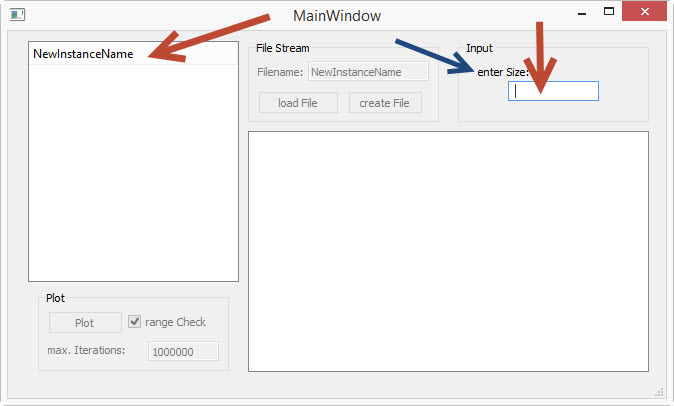
\includegraphics[width=1\linewidth]{./Pictures/MainWindow_createFile}
		\caption[erstelle Datei]{Nach Klick auf "{}create File"{} werden die neuen Parameter einzeln abgefragt}
		\label{fig:MainWindow_createFile}
	\end{figure}
	
	Nach erfolgreichem Einlesen aller Parameter wird die neue Instanz geladen und nebenstehend angezeigt.
	
	\begin{figure}[H]
		\centering
		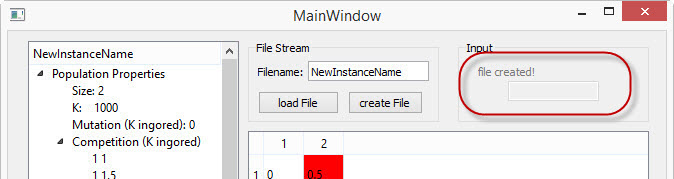
\includegraphics[width=1\linewidth]{./Pictures/MainWindow_FileCreated}
		\caption[Datei erstellt]{Nach Eingabe des letzten Parameters}
		\label{fig:MainWindow_FileCreated}
	\end{figure}
	
	\subsubsection{Darstellung des Graphen}
	Nach dem Erstellen oder Laden einer Testinstanz ist es möglich, die Simulation zu starten. Das erkennt man an dem aktivierten "{}Plot"{}-Bereich (vgl. Abb. \ref{MainWindow_Start}, zu \ref{Baumstruktur_geschlossen}, \ref{Baumstruktur_offen}, \ref{fig:MainWindow_FileCreated}) links unten.\\
	Wie man schon auf vielen Abbildungen zuvor beobachten kann, gibt es im "{}Plot"{}-Bereich ein Eingabefeld mit dem Titel "{}max. Iterations:"{} und ein Auswahlkästchen für "{}range Check"{}.\\
	Das Feld mit den "{}max. Iteraterions"{} gibt der Simulation vor, wie viele Sprünge zugelassen sind bis die gesammelten Populationsgrößen und die dabei vergangene Zeit gezeichnet werden. \\
	Mit dem Kästchen "{}range Check"{} erlaubt man der Simulation in günstigen Situationen schon vor Erreichen der maximalen Iterationszahl abzubrechen. Eine Situation wird als günstig eingestuft, sobald die Entfernung jedes Merkmals zu seinem Gleichgewicht an einem Punkt gering genug gewesen und etwas zusätzliche Zeit verstrichen ist. Die frühzeitigen Abbruchbedigungen skalieren mit der bereits verstrichenen Zeit und dem verwendeten K.\\

	Nach Absprache mit Loren Coquille und Martina Baar wurde von der graphischen Darstellung folgendes gewünscht:\\
	\begin{itemize}
		\item Man soll den zeitlichen Verlauf der Populationsgrößen beobachten \- können.
		\item Um die Prozesse besser analysieren zu können, soll es möglich sein, Stellen des Graphen näher betrachten zu können (zoom).
		\item Um Simulationen vergleichen zu können, sollen außerdem Ausschnitte als Bilder gespeichert werden können.
		\item Und natürlich soll das Programm bei der Berechnung nicht abstürzen.
	\end{itemize}
	Der letzte Punkt scheint vielleicht absurd, jedoch ist er bei der "{}Ereignisgesteuerten Programmierung"{} eine Hürde, die gemeistert werden muss.\\
	Im Gegensatz zur Konsolenanwendung, die alle Abläufe in einer festen Reihenfolge bearbeitet, entstehen Konflikte, wenn während einer Berechnung auf ein laufendes Programm zugegriffen wird. Die Reaktionen können nicht nebeneinander laufen, weil sie oft auf dieselben Ressourcen zugreifen. Das zwangsläufige Ergebnis hat wahrscheinlich jeder schon erlebt:
	\begin{figure}[H]
		\centering
		
\includegraphics[width=0.7\linewidth]{./Pictures/KeineRueckmeldung}
		\caption[Keine Rueckmeldung]{Hauptthread wurde überlastet}
		\label{Keine Rueckmeldung}
	\end{figure}
	Die Lösung dieses Problems ist, die aufwändige Berechnung auf einen getrennten Prozess auszulagern. Hier kommt die Unabhängigkeit der Module besonders gelegen, denn man kann die Verwendung der Ressourcen leicht organisieren.\\
	Die Auslagerung von Prozessen fällt unter den Begriff "{}Multithreading"{} und erstellt an geeigneter Stelle einen "{}Thread"{}, um ihm Aufgaben zuzuteilen. Sobald der Thread seine Arbeit erfüllt hat (Simulation des Prozesses), sendet er ein Signal, das vom Programm als Ereignis (wie Benutzereingabe) interpretiert wird, um (in unserem Fall) das Zeichnen der Daten zu initialisieren.\\
	Auf diese Weise nimmt das Programm (beide Fenster) weiter Benutzereingaben entgegen ohne seine Berechnungen unterbrechen zu müssen.\\
	Das Drücken der "{}Plot"{}-Schaltfläche öffnet das "{}Plot-Fenster"{} (Abbildung \ref{PlotWindow_start}).
	\begin{figure}[H]
		\centering
		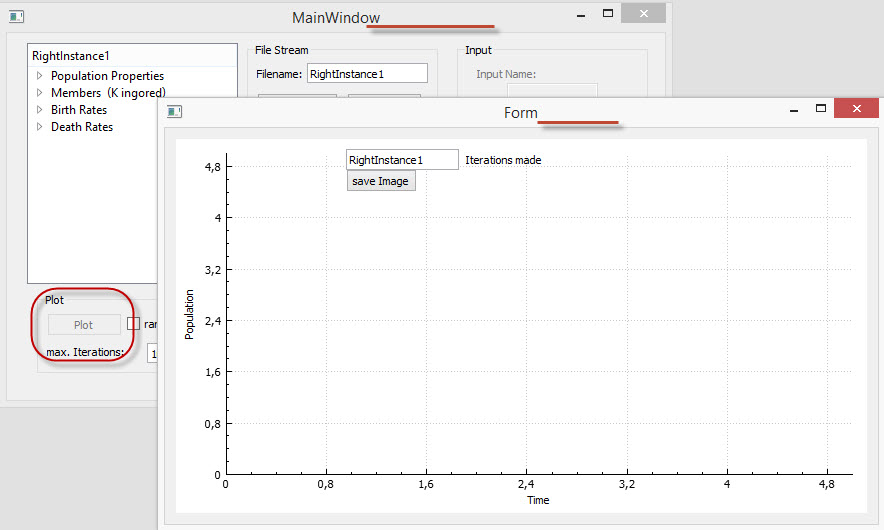
\includegraphics[width=1\linewidth]{./Pictures/PlotWindow_start}
		\caption[PlotWindow_start]{Start des PlotWindow}
		\label{PlotWindow_start}
	\end{figure}
	In blau sieht man, dass das Programm durch Übereinanderlegen während der Berechnung weiterhin ansprechbar ist statt keine Rückmeldung zu liefern (vgl. Abb. \ref{Keine Rueckmeldung}).\\
	Wenn die Simulation  einen günstigen Zustand erreicht oder die maximale Anzahl an gewünschten Iterationen absolviert hat, werden anschließend maximal 10mio Punkte auf dem Koordinatensystem zu Graphen verbunden (Abbildung \ref{PlotWindow_smallBPDL}). 
	\begin{figure}[H]
		\centering
		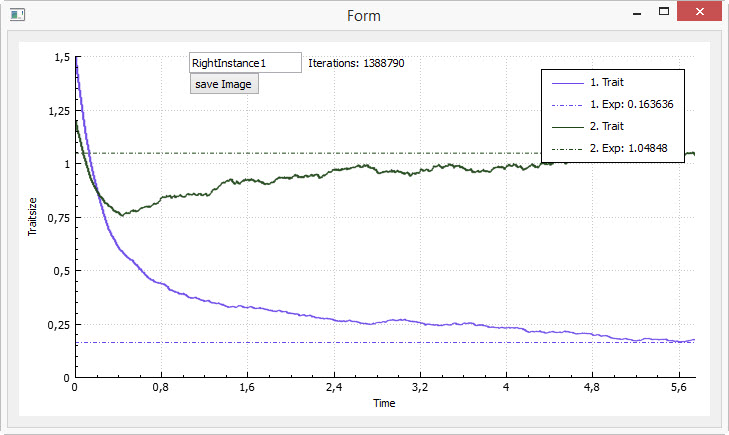
\includegraphics[width=0.9\linewidth]{./Pictures/PlotWindow_smallBPDL}
		\caption[PlotWindow]{PlotWindow mit Dimorpher Population}
		\label{PlotWindow_smallBPDL}
	\end{figure}
	
	Welche Optionen finden sich auf diesem Fenster?\\
	\begin{itemize}
		\item Natürlich kann man wie gewünscht in einem Koordinatensystem die zeitliche Entwicklung der Population verfolgen.
		\item Darüber hinaus sieht man in gestrichelten Linien die stabilen Zustände der Population und kann die Konvergenz dahin verfolgen.
		\item Außerdem ist bei aktiviertem "{}range Check"{} nicht klar, wie viele Iterationen (Sprünge) tatsächlich gemacht wurden, um den aktuellen Zustand zu erreichen. Zu diesem Zweck ist mittig im Bild ein Label "{}Iterations: "{}, worin der Wert 1388790 zu sehen ist.
		\item In der rechten oberen Ecke findet sich außerdem eine Legende der dargestellten Graphen. Dort sind im Wechsel die Merkmale mit ihrem erwarteten Gleichgewicht. "{}Exp"{} steht für "{}Expected"{} und kennzeichnet den Gleichgewichtszustand.
		\item Des weiteren findet sich eine Schaltfläche "{}save Image"{} und eine Textbox, in die man den gewünschten Bildnamen eintragen kann. Damit lässt sich das Bild mit Legende als .pdf und .jpg abspeichern.
	\end{itemize}

	Was man zwar nicht direkt in Abbildung \ref{PlotWindow_smallBPDL} sehen kann, aber gut ausgearbeitet wurde, ist die Bewegungsfreiheit auf dem Bild.\\
	\begin{itemize}
		\item Mann kann in das Bild hineinzoomen.
		\item Die Messgitter werden beim zoomen automatisch angepasst.
		\item Auf dem Koordinatensystem kann man sich durch "{}Ziehen"{} bewegen.
		\item Das Fenster lässt sich durch Strecken skalieren, wobei sich der Graph automatisch anpasst.
	\end{itemize}
	Als Beispiel dient Abbildung \ref{PlotWindow_zoomedBPDLmaximized}, welche durch Heranzoomen und Bewegen sowie maximierte Fenstergröße (vgl. kleine Legende) erstellt wurde.
	\begin{figure}[H]
		\centering
		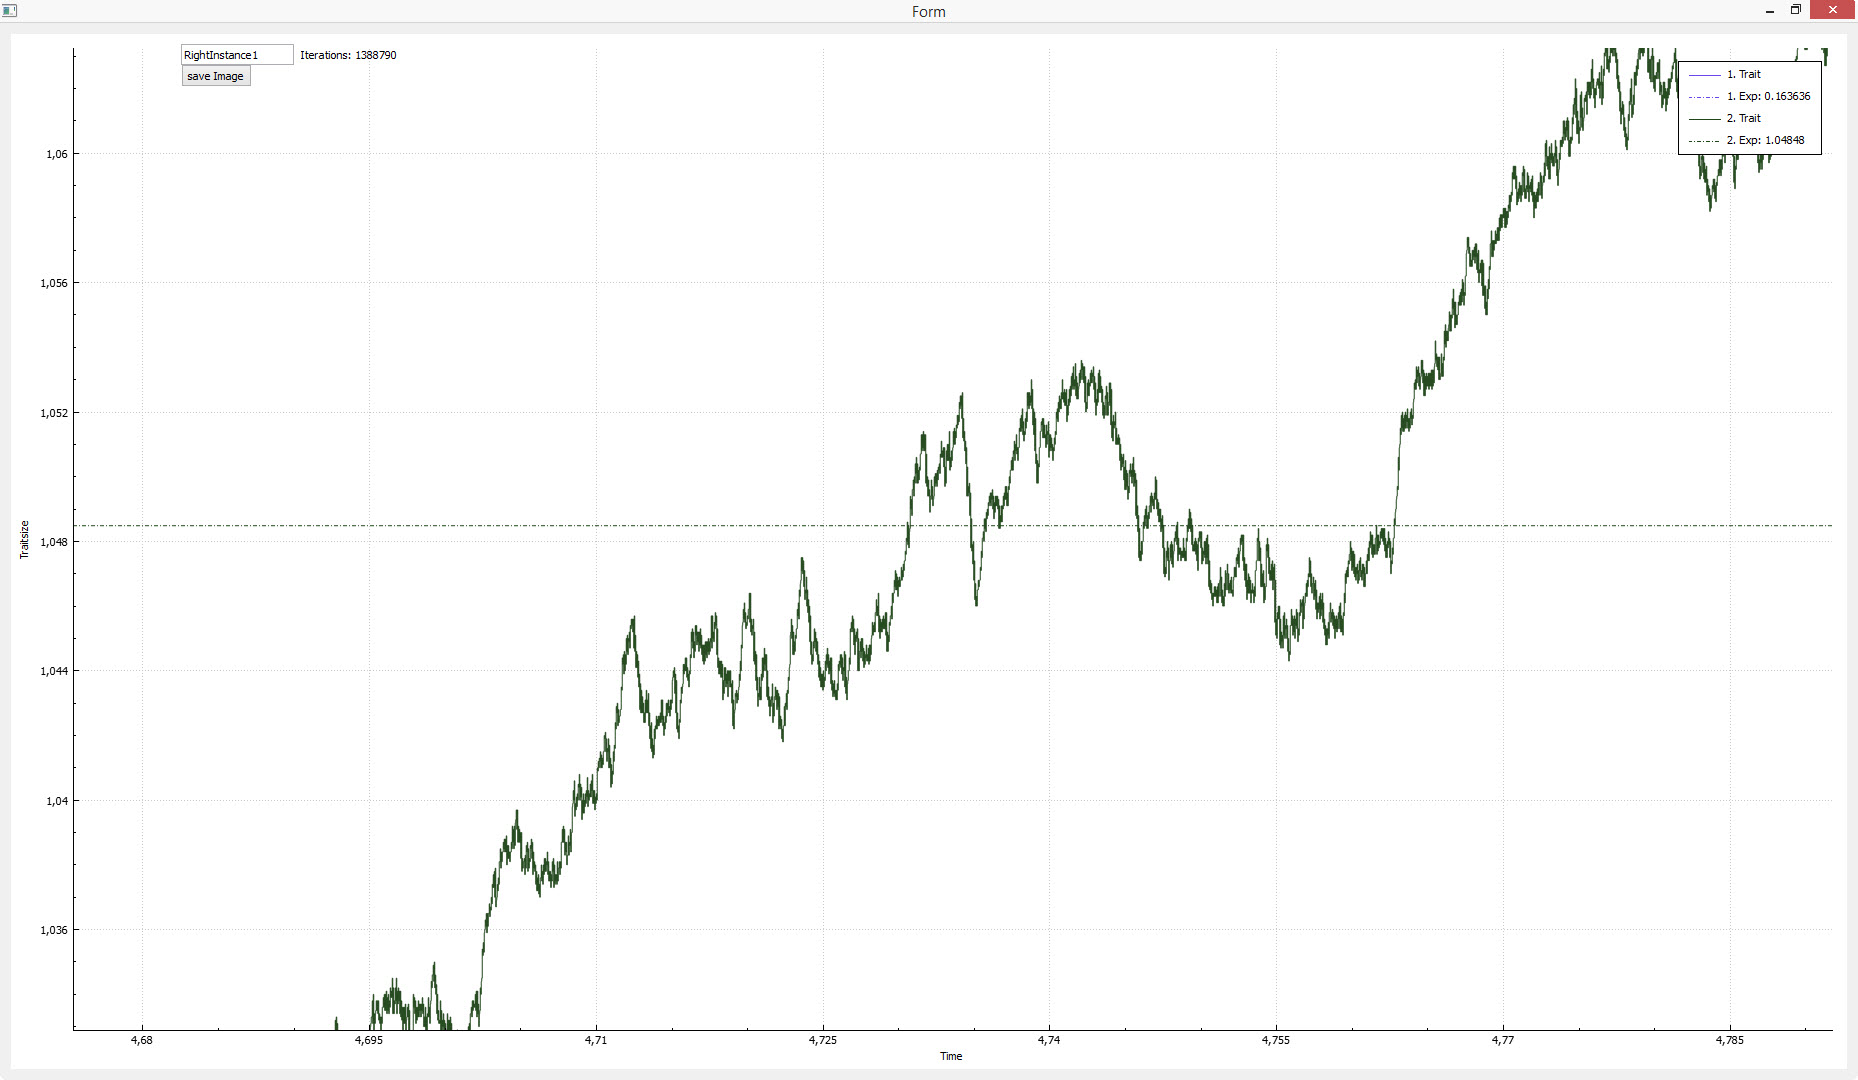
\includegraphics[width=1\linewidth]{./Pictures/PlotWindow_zoomedBPDLmaximized}
		\caption[PlotWindow]{PlotWindow mit Dimorpher Population}
		\label{PlotWindow_zoomedBPDLmaximized}
	\end{figure}
	Man kann sogar soweit skalieren, bis die Ereignisse lokal zählbar werden und der Plot eine Größe hat, in der das Messgitter eine Sprungmaschenweite hat:
	\begin{figure}[H]
		\centering
		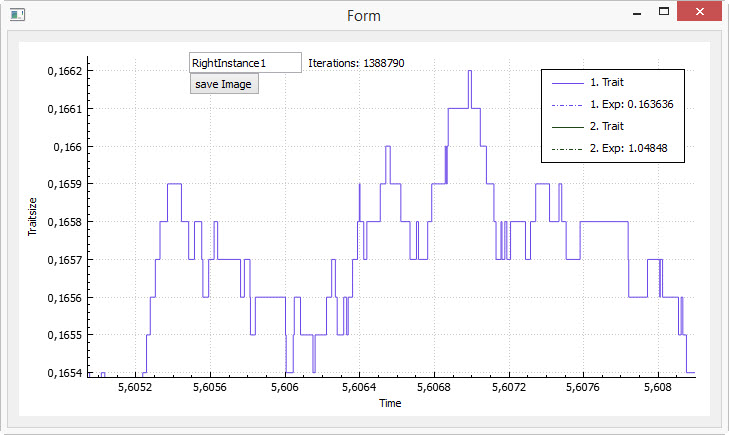
\includegraphics[width=1\linewidth]{./Pictures/PlotWindow_zoomedBPDL_Stepview}
		\caption[PlotWindow]{PlotWindow mit Dimorpher Population}
		\label{PlotWindow_zoomedBPDL_Stepview}
	\end{figure}	
	

\section{Verhaltenstests und Korrektheit der \\Implementierung}
Um beurteilen zu können, ob das erstellte Simulationsprogramm tatsächlich geeignet ist, ist es wichtig, die Korrektheit der Implementierung zu über\-prüfen. Dies gestaltet sich bei steigender Komplexität generell immer schwieriger (besonders bei zufallsbedingten Simulationen) und ist deswegen ein besonders interessantes Thema. Daher habe ich nach dem Prinzip der "{}testgetriebenen Entwicklung"{}  (Test Driven Develeopment - TDD) gearbeitet \cite{martin2007professionalism}.\\
Wie der Name schon verrät, geht es darum seine Entwicklung durch Tests, sogenannte "{}Unit Tests"{} anzutreiben. Diese Tests gewährleisten kontrollierte Bedingungen, um Änderungen und Funktionalität so souverän wie möglich zu gestalten.\\
Das Konzept des TDD kann durch die Zusammenarbeit dreier Punkte aus \cite{martin2008clean} gut beschrieben werden:
\begin{itemize}
	\item[\textbf{1.}] Produktiver Code sollte nur geschrieben werden, um einen fehlgeschlagenen Unit Test bestehen zu lassen.
	\item[\textbf{2.}] Ein Unit Test sollte nur soweit entwickelt werden, bis er fehlschlägt.
	\item[\textbf{3.}] Es sollte nur so viel produktiver Code geschrieben werden, um einen Unit Test bestehen zu lassen. \label{3Punkte}
\end{itemize}

	\subsection{Unit Tests}
	Was ist ein Unit Test und was tut er?\\
	Ein Unit Test ist nichts anderes als eine Funktion, die speziell dafür geschrieben wird, um ein implementiertes Verhalten bzgl. dem erwarteten Verhalten zu testen.\\
	Auf diese Weise würde nach den obigen drei Punkten z.B. zunächst eine Funktion (ein Test) geschrieben werden, die unser Modell mit Parametern initialisiert und prüft, ob die Geburtenrate für diese Parameter gleich dem erwarteten Wert ist. Erst dann würde eine Geburtenraten-Funktion geschrieben werden, die den Test bestehen lässt.\\ 
	Auf diese Weise lässt sich oft eine deutlich effizientere Programmstruktur modellieren, als man es ursprünglich geplant hatte. Das Planen ist natürlich trotzdem ein wesentlicher Schritt. Mehr Einzelheiten zur Effizienz finden sich in \cite[The Bowling Game: An example of test-first pair programming]{martin2008clean}.\\
	In der Abbildung \ref{Unit Test} ist ein Beispiel für eine Implementierung eines einfachen Tests, der prüft, ob alle Parameter korrekt aus der Datei in die Objekte geschrieben werden.\\
	Dazu werden in einer Schleife erst 1.000.000 mal immer wieder neu die Todesraten berechnet und schließlich geprüft ob alle Raten trotzdem dem erwarteten Wert entsprechen (roter Kasten). Das ist dank der modularen Implementierung, die in Kapitel 4 vorgestellt wurde, möglich.
	\begin{figure}[H]
		\centering
		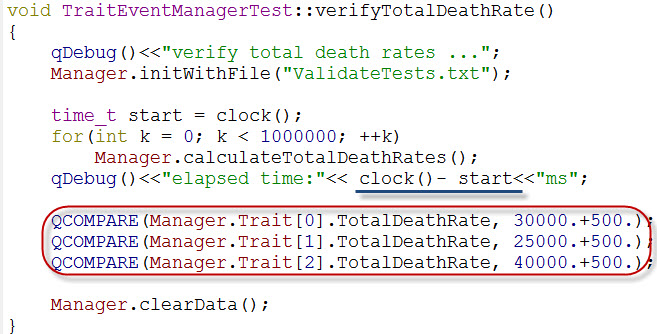
\includegraphics[width=1 \linewidth]{./Pictures/UnitTest_death}
		\caption[UnitTest]{UnitTest versichert korrekte Berechnung der Todesraten}
		\label{Unit Test}
	\end{figure}
	Startet man nun das Testprogramm, so werden der Reihe nach alle implementierten Tests gestartet. Die Ausgabe enthält Erfolge, Fehlschläge und zusätzliche Debug-Ausgaben. Das ist in Abbildung \ref{Test Results} für die ersten Tests des BPDL Programms vorgeführt worden. In rot sieht man den zuvor erwähnten Test:
	\begin{figure}[H]
		\centering
		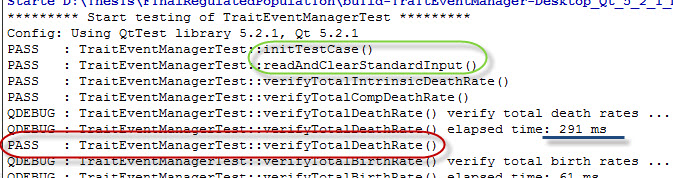
\includegraphics[width=1 \linewidth]{./Pictures/TestResult_start_death}
		\caption[Test Resultat einer Test Datei]{Ergebnisse einiger Tests}
		\label{Test Results}
	\end{figure}
	In blau sieht man, dass auch der praktische Aufwand gemessen wurde um Schwachstellen in der Implementierung aufzudecken (z.B. auch beim Ziehen von Zufallsvariablen).\\
	
	\subsubsection{Korrektheit durch Unit Tests}
	Warum sollten ein paar Tests für spezifische Situationen den Anspruch erheben Korrektheit des Programms zu gewährleisten?\\
	Das Besondere an unserer Simulation ist, dass zufälliges Verhalten vorliegt und daher kleinere Fehler oft nicht so einfach aufgedeckt werden können. Z.B. würde es in einer dimorphen BPDL Simulation nicht auffallen, wenn die Mutation unberücksichtigt bleibt, solange die Wahrscheinlichkeit gering ist, oder wenn die Zeiten zwischen Sprüngen nicht richtig sind. Gerade deswegen wurde die "{}Testgetriebene Entwicklung"{} so interessant.\\
	Die Korrektheit eines Programmkerns nachzuweisen kann sich als schwierig herausstellen, weil man die Korrektheit nicht für eine spezifische Instanz, sondern flexibel für alle nachweisen möchte. Doch ist es nicht notwendig die Flexibilität des Programms zu testen, wenn man stattdessen versucht, die Korrektheit jedes Arbeitsschrittes zu prüfen. Ein Arbeitsschritt erhebt in unserem Fall keinen Anspruch auf Komplexität. Tatsächlich sind unsere Arbeitsschritte alle möglichst einfach und erfüllen nur eine Aufgabe. D.h. die Korrektheit der Arbeitsschritte zu verifizieren lässt sich denkbar einfach mit einem Test abdecken.\\
	Wenn nun jeder Arbeitsschritt seine Aufgabe nachweisbar richtig erfüllt, dann kann davon ausgegangen werden, dass durch richtige Verwendung der Arbeitsschritte das erwartete Verhalten eintritt. Die richtige Verwendung der Arbeitsschritte wird dadurch einfach nachzuweisen, dass wir in Kapitel 4 den Algorithmus für einen Evolutionsschritt vorgestellt haben. Dass dieser eine Schritt richtig ausgeführt wird, ist anhand des Pseudocodes leicht ersichtlich. Doch ist der nächste Schritt nichts anderes als der erste Schritt, nur mit leicht veränderten Startwerten. Wenn also die Startwerte korrekt sind, dann wird auch der nächste Schritt wieder richtig ausgeführt.\\
	Auf diese Weise wird die Komplexität der Simulation vereinfacht auf die der Ablaufpunkte, die im Wesentlichen sehr einfach sind.\\
	Was allerdings nicht geprüft wurde, ist der Umgang mit den erhobenen Daten innerhalb des "{}GUI"{}-Moduls. Aufgrund des zeitlichen Rahmens der Arbeit war es nicht mehr möglich, eine Methode zum Test von ereignisgesteuertem Code zu recherchieren und anzuwenden, sodass nur zwei von den drei in Abbildung \ref{Module und Klassen} beschriebenen Modulen getestet werden konnten.

	\subsection{Unit Tests des Programmkerns}
	Hier werden Tests vorgestellt, mit denen die korrekte Berechnung der Raten verifiziert werden soll. Dazu wird die folgende Testinstanz mit drei Merkmalen ($ X = \{x,y,z\} $) verwendet:\\
	\begin{center}
		\begin{minipage}{0.35 \textwidth}
			\begin{tabular}{ c | c c c }
			 $ c(\cdot, \cdot) $ & x & y & z \\
			 \hline
			 x & 2 & 1 & 0 \\
			 y & 0 & 2 & 0.5 \\
			 z & 0 & 2 & 2 \\
			\end{tabular}
			\end{minipage}
			\begin{minipage}{0.5 \textwidth}
			\begin{tabular}{ c | c  c  c  c  c  c  c }
			 & $ b(\cdot ) $ &  & $ d(\cdot ) $ & & $ n(\cdot ) $ & & $ \mu $\\
			 \hline
			 x & 10 &  & 5 & & 100 & & 0.1\\
			 y & 10 &  & 5 & & 100 & & 0.1\\   
			 z & 10 &  & 5 & & 100 & & 0.1\\
			\end{tabular}
			\end{minipage}
	\end{center}
	Es wurden drei Merkmale gewählt, weil dies die minimale Anzahl ist, um die Auswirkungen von "{}inneren"{} Merkmalen auf Rand-Merkmale (und umgekehrt) zu testen.\\
	Vor den Kerntests wurden noch Tests gemacht, die versichern, dass kein Fehler beim Lesen, Schreiben, Neulesen, Verändern etc. der Raten und Parameter auftritt. Diese sind z.B. in grün in Abbildung \ref{Test Results} zu sehen.

	\subsubsection{Raten}
	Das Testen der Todesraten läuft auf den finalen Todesraten-Test aus Abbildung \ref{Unit Test} hinaus. Diese zeigt die Implementierung des entsprechenden Tests. Jede weitere Implementierung kann im Quellcode nachgesehen werden, jedoch werden hier nur heuristisch die Tests aufgelistet, um die Qualitätstests nachvollziehbar zu machen. In den Tests selbst werden stets jedes Merkmal und dessen Werte auf Korrektheit geprüft, obwohl folgend immer nur ein Merkmal vorgerechnet wird.\\
	
	\textbf{Intrinsische Todesrate:}\\
	Exemplarisch an $ y $ erwarten wir für diese Instanz folgende Berechnung:\\
	\renewcommand{\arraystretch}{1.2}
	\begin{tabular}{c l}
		\underline{Erwartet}: 		& $ d(y) \cdot n(y)  $\\
						& $ = 5 \cdot 100 = 500 $ \\\\
		\underline{Testergebnis}: 	& $ \trvec{500}{500}{500} $
	\end{tabular}\\\\
	Der Vergleich mit dem Testergebnis bestätigt somit das Verhalten der intrinsischen Todesraten-Berechnung.\\
	
	\textbf{Todesrate durch Wettbewerb:}\\
	Erneut an $ y $ erwarten wir für diese Instanz folgende Berechnung:\\
	
	\begin{tabular}{c l}
		\underline{Erwartet}: 		& $ n_0(y) \cdot \sum_{w \in X} c(y,w) \cdot n_0(w) $\\
						& $ = 100 \cdot ( 2 \cdot 100 + 0.5 \cdot 100 ) = 25000 $\\\\
		\underline{Testergebnis}: 	& $ \trvec{30000}{25000}{40000} $
	\end{tabular}\\\\
	Wie erwartet bestätigt sich das Ergebnis für $ y $. Durch den großen Abstand zum Equilibrium beider Funktionen entsteht hier natürlich eine große wettbewerbliche Todesrate. Außerdem lässt sich beobachten, dass für das letzte Merkmal $ z $ die größte Rate berechnet wurde, was mit der Zeilensumme der Wettbewerbsmatrix begründet werden kann.\\
	
	\textbf{Totale Todesraten:}\\
	Hier muss nicht mehr viel vorbereitet werden. Wir haben bereits die intrinsische und wettbewerbliche Todesrate ausgerechnet. \\
	
	\begin{tabular}{c l}
		\underline{Erwartet}: 		& $ D(y) =  d(y) \cdot n(y) + n_0(y) \cdot \sum_{w \in X} c(y,w) \cdot n_0(w) $\\
						& $ = 500 + 25000 = 25500$\\\\
		\underline{Testergebnis}: 	& $ \trvec{30500}{25500}{40500} $
	\end{tabular}\\\\
	Wie erwartet bestätigt sich das Ergebnis für $ y $. In Abbildung \ref{Test Results} kann man die Ausführung aller drei Tests verfolgen.\\
	In anderen Tests (des TSS Programms) wurden dieselben Prüfungen noch für unterschiedliche Instanzen gemacht.\\
	
	\textbf{Totale Geburtenraten:}\\
	Hier wird exemplarisch erneut das mittlere Merkmal $ y $ verwendet, welches durch die Mutation von beiden Seiten eine höhere Geburtenrate erwartet. \\
	
	\begin{tabular}{c l}
		\underline{Erwartet}: 		& $ B(y) = (1-\mu) \cdot b(y) \cdot n_0(y) + \frac{\mu}{2} \cdot \left( \sum_{w \in X} b(w) \cdot n_0(w) \right) $\\
						& $ = 10 \cdot 100 + 0.05 \cdot (10 \cdot 100 + 10 \cdot 100) = 1000$\\\\
		\underline{Testergebnis}: 	& $ \trvec{950}{1000}{950} $
	\end{tabular}\\\\
	Die Geburtenraten unterscheiden sich nur zwischen Rand und Innerem um  $ 50 $, da wir die mutative Geburtenrate $ 0.05 \cdot 10 \cdot 100 = 50 $ von links und rechts an Randmerkmalen natürlich nur einmal erhalten.\\
	
	\textbf{Totale Raten:}\\
	Dank der vorherigen Schritte lässt sich die Totale Merkmalsrate leicht berechnen:\\
	
	\begin{tabular}{c l}
		\underline{Erwartet}: 		& $ B(y) + D(y) = $\\
						& $ 1000 + 25500 $, bzw. $ \trvec{950}{1000}{950} + \trvec{30500}{25500}{40500} = \trvec{31450}{26500}{41450} $\\\\
		\underline{Testergebnis}: 	& $ \trvec{31450}{26500}{41450} $
	\end{tabular}\\\\
	Schließlich folgt daraus auch die Totale Ereignisrate:\\
	
	\begin{tabular}{c l}
		\underline{Erwartet}: 		& $ 31450 + 26500 + 41450 = 99400 $\\\\
		\underline{Testergebnis}: 	& $ 99400 $
	\end{tabular}\\\\
	Das beendet die wesentlichen Tests zur Berechnung der Raten.
	
	\subsubsection{Ziehen einer Ereigniszeit}
	In diesem zweiten Teil der Tests werden Ereigniszeiten gezogen und mit dem Gesetz der großen Zahlen der Mittelwert mit dem erwarteten Mittelwert verglichen.\\
	Es gab noch weitere Tests, die hier nicht erwähnt werden, weil sie bloß testen, ob der verwendete "{}Würfel"{} wirklich unabhängige Ziehungen macht und ob die Verteilung das tut, was sie soll.\\
	
	\textbf{Geburts- und Todeszeitpunkte:}\\
	Um diese Ziehung zu verifizieren wurden $ 1.000.000 $ Ereigniszeitpunkte mit denselben Raten gezogen und gemittelt.\\
	Der Erwartungswert dieser Ziehung entspricht $ \frac{1}{\text{TotalEventRate}} $, was auch der Referenzwert für die Fehlerberechnung ist. Für das Testergebnis wird eine absolute Genauigkeit von $ 99.995 \% $ gefordert und der Fehler erreicht meistens einen Wert um $ 0.0008\% $.\\
	
	\textbf{TSS-Mutationszeiten:}\\
	Für die korrekte Ziehung der Mutationszeitpunkte in einer TSS-Simulation wird eine etwas andere Testinstanz verwendet, die nicht entscheidend ist, aber in allen TSS-Testinstanzen verwendet wird. Diese Instanz ist unter dem Namen "{}ValidateTSSTests.txt"{} im Programmordner zu finden und stellt sicher, dass die Fitness einen Wechsel der Merkmale garantiert.\\
	Um die Mutationszeiten zu validieren wird 100.000 mal der folgende Ablauf durchgegangen:
	\begin{itemize}
		\item[\textbf{1}] Zunächst werden alle bis auf ein Merkmal getötet.
		\item[\textbf{2}] Das übrige Merkmal wird auf sein Gleichgewicht gehoben.
		\item[\textbf{3}] Dann wird eine Funktion aufgerufen, die im nächsten Kapitel vorgestellt wird und den Zeitpunkt der nächsten Mutation aus den Mutationsraten zieht.
		\item[\textbf{4}] Dieser Zeitpunkt wird zu vorhergehenden Zeiten summiert.
	\end{itemize}
	Nach der Schleife wird das Mittel gezogen und auf eine absolute Genauigkeit von $ 99.95\% $ geprüft. Die Testergebnisse lagen in der Regel bei einem Fehler um $ 0.002\% $.\\
	
	\subsubsection{Veränderung der Population}
	Ich komme nun zum letzten Bereich der Aufteilung aus Abbildung \ref{fig:PseudoCodeForBThesis}, Ebene 1.\\
	
	\textbf{Merkmal auswählen}\\
	Um zu verifizieren, dass die Merkmale korrekt den Ereignissen zugeteilt werden, wurde ein Histogramm der Wahlen erstellt. Genau gesagt wurde 100.000 mal entschieden, welches Merkmal ein Ereignis auslösen wird.\\
	Wie schon in Kapitel 4 erwähnt, ist es sehr nützlich gewesen die Raten getrennt zu berechnen und zu speichern. Von diesem Vorteil kann jetzt Gebrauch gemacht werden, um zu unterscheiden welches Merkmal wie viele der 100.000 Ereignisse ausgelöst hätte.\\
	Die getestete Genauigkeit war $ 99.95\% $ und wie zuvor haben die Ergebnisse sie stets ausreichend überschritten.\\
	
	\textbf{Ereignistyp wählen}\\
	Die Idee dieses Tests ist praktisch identisch zum Vorherigen und wird nicht näher beschrieben, ist aber natürlich ausführlich im Quellcode vorhanden und hat ebenso bestanden.\\
	
	\textbf{Ereignis ausführen}\\
	Hier wurde getestet, ob das Ausführen eines gewählten Ereignisses auf ein gewähltes Merkmal korrekt abläuft. Dabei wurde lediglich geprüft, ob die Population bei einer Geburt wirklich anwächst und bei Tod bis zu einem Minimum von 0 sinken kann.
	
	\subsection{Unit Tests der Konvergenz}
	Hier wurde zunächst geprüft, ob das vom Programm ermittelte Gleichgewicht wirklich richtig berechnet wurde.\\
	Schließlich wurde für dimorphe und monomorphe Populationen getestet, ob und wie gut die Konvergenz für wachsende K zum Gleichgewicht abläuft. Hierzu wurden 1.000.000 Sprünge des Prozesses mit $ K = 10 $ und $ K = 10.000 $ gemacht. Für $ K = 10 $ bewegt sich der Fehler um $ 0.1\% $ und für $ K = 10.000 $ um $ 0.001\% $. Besonders bei großem $ K $ konnte man beobachten, dass der Fehler oft mit der dimorphen Population korreliert, d.h. beide vergleichbar gering oder hoch sind.
	
	
\section{TSS-Prozesse}
In diesem Kapitel geht es um TSS-Prozesse und wie eine Annäherung dieser durch unsere Simulation gelöst wurde.
	\subsection{Invasion}
	Wie schon im Rahmen der Fitnessfunktion angesprochen, beschreibt die Invasion den Vorgang, durch den ein neu auftretendes Merkmal (dank Mutation) ein bis dahin dominantes Merkmal verdrängt.\\
	In Kapitel 3.2 haben wir weiterhin gesehen, dass der BPDL-Prozess für $ K \to \infty $ gegen ein deterministisches System konvergiert. Jedoch soll unser TSS-Prozess ein nicht deterministischer Prozess sein, der eine monomorphe Population simuliert, die zu zufälligen Zeiten ihr dominantes Merkmal austauscht.\\
	Um dies zu erreichen wird der Grenzwert nicht nur mit $ K \to \infty $, sondern gleichzeitig $ \mu \to 0 $ gebildet. Auf diese Weise wird das sonst so deterministische Verhalten aus $ K \to \infty $ durch weiterhin zufällige Ereignisse beeinflusst.\\
	Dabei wird der aus Kapitel 3.6 bekannte Bereich (\ref{TSSMutation}) für die Konvergenz von $ \mu $ gewählt. Er garantiert, dass eine Invasion ausreichend Zeit zur Verdrängung hat, bis ein weiterer Mutant entsteht und nicht zu viel Zeit vergeht, sodass vor der nächsten Mutation die Population ausstirbt.\\
	Des Weiteren wollen wir sicherstellen, dass sich auf lange Sicht nur ein Merkmal durchsetzt. Dies können wir erreichen, in dem wir ausnutzen, dass stets zwei Merkmale um Dominanz streiten, und die Aussagen aus Kapitel 3.5 (Dimorphes Gleichgewicht) auf mehrere Merkmale ausweiten.\\
	Wenn für beliebiges $ x \in X $ und für alle $ y \in (X\backslash x) $ entweder $ f(y,x) < 0 $ oder $ f(y,x) > 0 $ und $ f(x,y) < 0 $, so ist sichergestellt, dass sich auf lange Sicht ein Merkmal in der Population durchsetzen wird und keine zwei Merkmale nebeneinander existieren können. Unter diesen Umständen können weiterhin die stabilen monomorphen Zustände, die in Kapitel 3.5 beschrieben wurden, angenommen werden, nur eben für mehrere Merkmale.\\
	
	\textbf{Welche Phasen durchläuft eine Invasion?}\\
	Damit ein Merkmal y ein dominantes Merkmal x verdrängen kann, muss nach obigen Erkenntnissen zunächst einmal $ f(y,x) > 0 $ und $ f(x,y) < 0 $ gelten.\\
	Wie aus \cite{Silke} beschrieben, lässt sich die Invasion in drei Teilen beschreiben. 
	\begin{itemize}
		\item [1.] Fixierung: Zu Beginn einer Invasion werden die Individuen des Merkmals $ x $ kaum von $ y $ beeinflusst, da $ c(x,y)n(y) $ unbedeutend klein ist. Jedoch ist dieser Zustand zeitlich durch die positive Wachstumsrate des Merkmals $ y $ für $ x $ im Gleichgewicht $ \bar{n}_x $ begrenzt. Ab einer bestimmten Populationsgröße $ \eps $, kann der Einfluss des Eindringlings $ x $ von $ y $ nicht mehr ignoriert werden. Die Dauer, bis ein erster Mutant das Merkmal zu diesem relevanten Niveau bringt, hat die Größenordnung $ \log K $.
		\item [2.] Invasion: Hier ereignet sich der Fall des dominanten Merkmals $ x $ und der Anstieg des neuen Merkmals $ y $. Dank $ f(x,y) < 0 $ und $ f(y,x) > 0 $ beobachten wir die Konvergenz gegen das neue Gleichgewicht $ (0,\bar{n}_y) $.
		\item [3.] Aussterben: Hier greift der umgekehrte Fall der Fixierung. Sobald $ n(x) < \eps $ geworden ist, kann zunächst der Einfluss von $ x $ auf $ y $ vernachlässigt werden. Dank der negativen Wachstumsrate wird das Merkmal $ x $ in einer Zeit von der Ordnung $ \log K $ aussterben.
	\end{itemize}
	Beispielhaft kann man das an folgenden Abbildungen beobachten:\\
	\begin{minipage}{0.7 \textwidth}
	\begin{figure}[H]
		\centering
		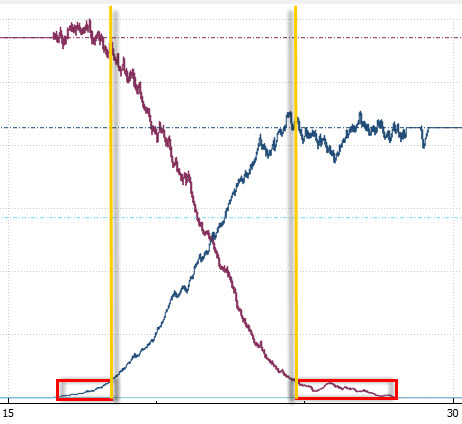
\includegraphics[width=1 \linewidth]{./Pictures/Invasion2}
		\caption[Invasion]{Eine Invasion für K = 1000}
		\label{Invasionsphasen}
	\end{figure}
	\end{minipage}
	\begin{minipage}{0.3 \textwidth}
		In rot sind die Fixierungsphasen gekennzeichnet und in orange erkennt man die Zeitpunkte, an denen die Übergänge beobachtbar sind.
	\end{minipage}\\
	
	Man kann in dieser Stelle bereits erahnen, dass die Fitnessfunktion bzw. die Wachstumsrate eines Mutanten die Möglichkeit bietet, Aussagen über die Invasionswahrscheinlichkeit zu machen. Und tatsächlich erhalten wir aus \cite{Champagnat20061127}, dass die Invasionswahrscheinlichkeit mit $ K \to \infty $ gegen
	\[ \frac{\left[ f(y,x)\right]_+ }{b(y)} \]
	konvergiert.
	
	\subsubsection{Praktische Umsetzung}
	Normalerweise lassen sich die Parameter einer Simulation so wählen, dass bei mindestens drei Merkmalen ein Kreislauf der Invasionen erzwungen werden kann. D.h. es wird nicht dazu kommen, dass ein Merkmal nicht verdrängt werden kann, also: $ x \xleftarrow{verdr"angt} y \xleftarrow{verdr"angt} z \xleftarrow{verdr"angt} x \dots $\\
	In unserem Modell jedoch haben wir nur Mutationen zu den Nachbarn erlaubt. Diese Einschränkung verhindert den Kreislauf. Wenn ein Merkmal $ y $ ein $ x $ verdrängt, so kann es nicht mehr von selbigem $ x $ verdrängt werden, sondern muss vom anderen Nachbarn verdrängt werden.\\
	Auf diese Weise wandert die Vorherrschaft in der Population, bis ein Merkmal dominant ist, welches keine fitteren Nachbarn hat oder am Rand angekommen ist, was zwangsläufig wieder dem vorherigen Fall entspricht.\\
	Die Darstellung der Fitnessmatrix im Programm lässt sich an folgendem Bild leicht nachvollziehen:
	\begin{figure}[H]
		\centering
		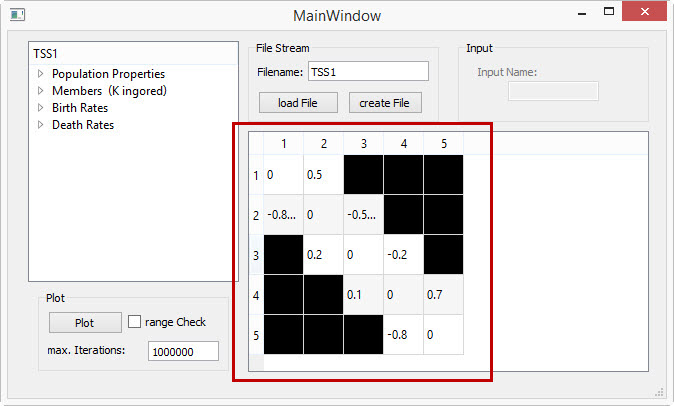
\includegraphics[width=1\linewidth]{./Pictures/MainWindow_BandMatrix}
		\caption[Fitness Matrix]{Fitness Bandmatrix}
		\label{MainWindow mit Fitness Bandmatrix}
	\end{figure}
	Da die Fitness nicht die einzige nützliche Information bei Invasionen ist, wurde dem Programm noch die Möglichkeit gegeben, farblich darauf hinzuweisen, ob Invasion möglich und ob sie besonders wahrscheinlich ist.\\
	Dazu folgendes Bild:
	\begin{figure}[H]
		\centering
		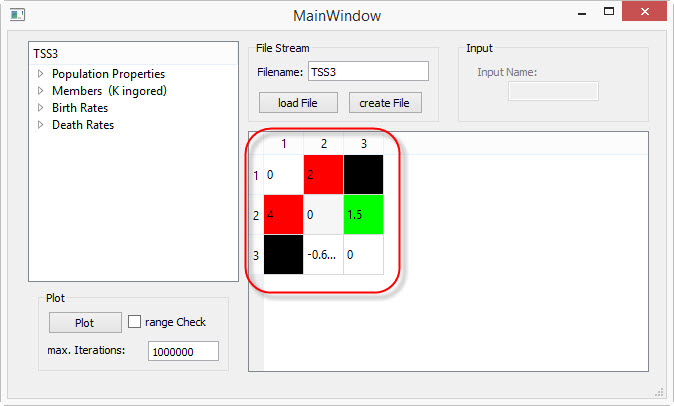
\includegraphics[width=1\linewidth]{./Pictures/MainWindow_red_green_loaded}
		\caption[MainWindow_redGreenFitness]{Fitness Matrix mit roten und grünen Akzenten}
		\label{fig:MainWindow_red_green_loaded}
	\end{figure}
	Dabei werden drei Farben unterschieden. 
	\begin{itemize}
		\item [\textbf{Rot}] werden beide Merkmale gefärbt, falls wir einen Zustand der Koexistenz erwarten. In diesem Fall sind $ f(x,y) \& f(y,x) > 0 $.
		\item [\textbf{Weiß}] wird ein Merkmal gefärbt, wenn es verdrängen oder verdrängt werden kann.
		\item [\textbf{Grün}] wird ein Merkmal gefärbt, wenn die Verdrängungswahrscheinlichkeit über 60\% ist.
	\end{itemize}

	\subsection{Optimierung}
	Einfach den BPDL-Simulator zu verwenden, um diesen Grenzwertprozess zu approximieren, würde darin resultieren, dass sehr viel Rechenzeit im Gleichgewicht eines Merkmals verbracht werden würde.\\
	Die Beobachtung des Prozesses im Gleichgewicht ist nicht besonders interessant und es lässt sich dabei nicht gut nachvollziehen, wann vielleicht Mutanten Invasionsversuche gestartet haben, die sich nicht behaupten konnten. Diese Simulation wurde bereits in Abbildung \ref{TSS_mitBPDLSimulator} vorgestellt.\\
	Alternativ wird hier eine andere Variante dieser Simulation vorgestellt. 
	Diese nutzt eine lineare Interpolation als eine Optimierung um die Übersichtlichkeit, Analysefähigkeit und Laufzeit deutlich zu verbessern.\\
	Diese lineare Interpolation macht es notwendig, stets zu wissen in welcher der drei Phasen der Prozess sich zur Zeit bewegt. Sobald er die Aussterben-Phase verlassen hat und schließlich der Prozess sein Equilibrium erreicht, wird eine Interpolation des Prozesses bis zu seiner nächsten Mutation durchgeführt.\\
	Die Sprünge bis zum nächsten Mutanten werden nicht berechnet, stattdessen wird anhand der Geburtenrate der toten Nachbarn eine Mutationsrate zusammengefasst, welche uns die Zeit für die nächste Mutation liefert. Danach wird nach dem selben Vorgehen, wie in Kapitel 4 beschrieben, entschieden, welcher Nachbar die Mutation ausgelöst hat.\\
	\begin{figure}[H]
		\centering
		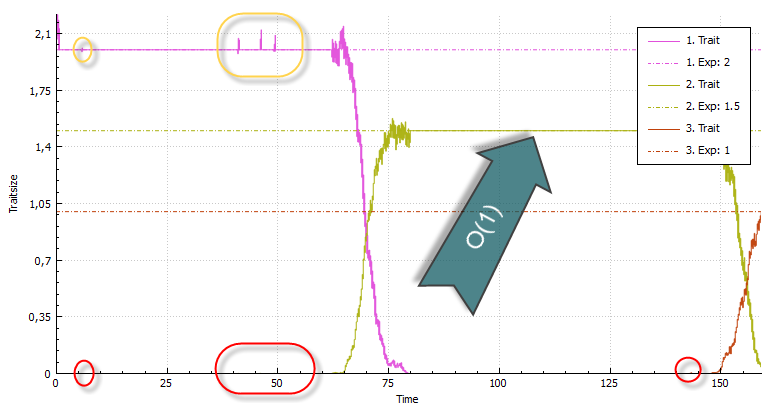
\includegraphics[width=1\linewidth]{./Pictures/TSS2_optimierung_small}
		\caption[MainWindow_redGreenFitness]{optimierte Simulation einer TSS-Approximation}
		\label{TSS2_optimierung_small}
	\end{figure}
	Dass sich dadurch die größte Rechenzeit auf $ O(1) $ verkürzt und die Über\-sichtlichkeit verbessert, ist sehr deutlich und war zu erwarten. Die Analysemöglichkeiten jedoch verbessern sich dank des großen Ratenunterschiedes der Merkmale. Der eindringende Mutant bietet dem neuen Merkmal nur eine sehr geringe Ereignisrate. Während dieser Zeit sind große Bewegungen im dominanten Merkmal zu erwarten. Diese Beobachtung lässt sich leicht in Abbildung \ref{TSS2_optimierung_small} nachvollziehen, wo man in rot niemals einen Mutanten entdecken würde, jedoch dank der Ausschläge in der gelben Markierung ist es einfach die Mutanten aufzuspüren.\\
	Folgend werden beide Effekte gegenübergestellt:\\
	\begin{center}
	\begin{minipage}{1\textwidth}
	\begin{minipage}{0.25\textwidth}
		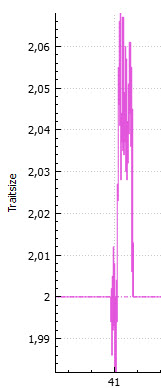
\includegraphics[width=1\linewidth]{./Pictures/TSS_DomZoomVgl_original}
	\end{minipage}
	$ \quad $
	\begin{minipage}{0.25\textwidth}
		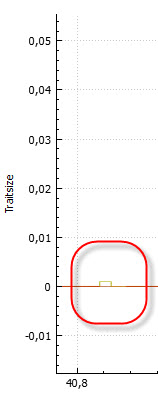
\includegraphics[width=1\linewidth]{./Pictures/TSS_MutationZoomVgl2_original}
	\end{minipage}
	$ \quad $
	\begin{minipage}{0.28\textwidth}
		Dank der Beweglichkeit auf dem Koordinatensystem ist es möglich,  die Entwicklung des Mutanten näher zu betrachten (nebenstehendes Bild). Oder man kann die Invasionsversuche aufspüren und auf eine deutliche Skala bringen (unteres Bild).
%		Natürlich ist es dank der Beweglichkeit auf dem Graphen auch möglich, die Entwicklung des Mutanten näher zu betrachten:
	\end{minipage}
	\end{minipage}
	\end{center}	
%	Natürlich ist es dank der Beweglichkeit auf dem Graphen auch möglich, die Entwicklung des Mutanten näher zu betrachten:
	\begin{figure}[H]
		\centering
		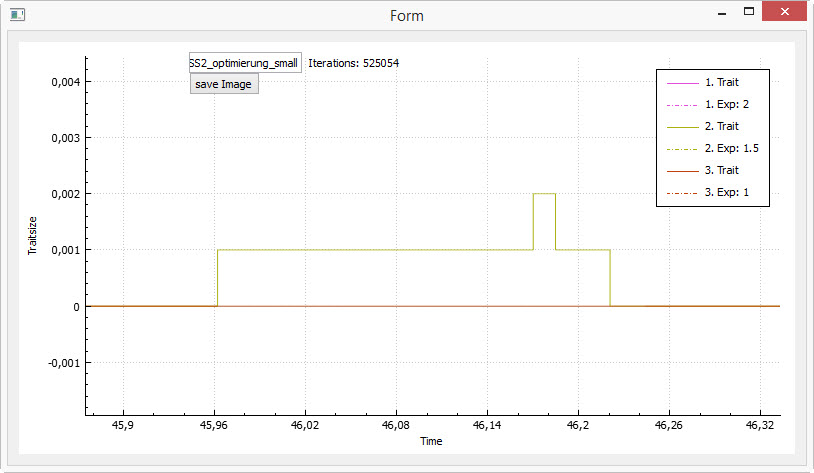
\includegraphics[width=1\linewidth]{./Pictures/TSS_MutationZoom2_original}
		\caption{Dritte Mutation von Links}
		\label{TSS_MutationZoom2_original}
	\end{figure}
	
	\subsection{Implementierung}
	Welche Form die Implementierung und der Algorithmus annehmen, wurde bereits in Kapitel 4 ausreichend erläutert. Deswegen wird hier nur kurz erklärt, wie sich der Algorithmus ändern würde. Die tatsächliche Implementierung weicht etwas ab und verwendet technisch unwichtige Details.\\
	
	Die Implementierung benötigt jetzt, bevor sie einen gewöhnlichen Sprung macht, zusätzlich eine Überprüfung, ob wirklich ein Prozesssprung oder eine Interpolation ausgeführt werden soll.\\
	Dazu wird nach jedem Sprung eine Abfrage "{}isNear()" gestartet, die prüft, ob es nur ein lebendes Merkmal gibt und ob dieses im Gleichgewicht ist:
	\begin{algorithm}[H]
		\caption{isNear()}
		\begin{algorithmic}[1]
			\Ensure{Bedingungen für eine Interpolation}
			\For{ i = 0 $ < $ n-1}
				\If{i $ \ne $ ChosenTrait \& Members[i] $ > 0 $}
					\State \Return false;
				\EndIf
			\EndFor
			\If{$ |\text{getKMembersOf[i]} - \text{Expected[ChosenTrait]}| > \frac{0.5}{K} $}
				\State \Return false;
			\EndIf
			\State \Return true;
		\end{algorithmic}
	\end{algorithm}
	Hier sorgt Zeile 2 in der Schleife dafür, dass außer dem zuletzt aktiven kein weiteres Merkmal aktiv sein könnte.\\
	Danach wird in Zeile 6 sicher gestellt, dass der Abstand zum Gleichgewicht minimal ist. Das ist notwendig, da der minimale Abstand nicht immer $ 0 $ ist. Falls das Gleichgewicht einen Wert ergibt, der kein Vielfaches von $ \frac{1}{K} $ ist, so kann das Gleichgewicht nicht durch den Prozess angenommen werden. In diesem Fall wird der Prozess jedoch stattdessen einen Sprungpunkt im Radius $ \frac{0.5}{K} $ um das Gleichgewicht haben.\\
	Als Abbruchkriterium wird nicht mehr einfach die maximale Anzahl erlaubter Sprünge verwendet, sondern auch ein Interpolationspunkt des Merkmals, an dem keine fitteren Nachbarn mehr vorhanden sind. Die Implementierung des Abbruchkriteriums sollte intuitiv sein und wird deshalb nicht weiter beschrieben.\\
	
	\textbf{Aufwand}\\
	Eine Besonderheit lässt sich zum Schluss noch betonen. Durch die Interpolation ist der Aufwand der Berechnung nicht mehr allein von K abhängig, sondern besonders von der Anzahl der erwarteten Mutationen und der Anzahl der erwarteten Invasionen.
	

\section{Schlusswort}
\subsection{Ausblick}
Schon früh war klar, dass noch viele Möglichkeiten offen bleiben werden, wie die Simulation erweitert werden kann. Einige größere Anpassungen, von denen auch welche nach dem Erstellen dieser Arbeit umgesetzt werden, werden hier kurz vorgestellt:
\begin{itemize}
	\item[1.] Dank der hier verwendeten Art der Implementierung ist das Erweitern des Programmkerns auf alternative Modelle denkbar einfach. So wäre es sehr einfach die Mutationswahrscheinlichkeit nicht nur mit gleichen Teilen auf die Nachbarn zu verteilen, sondern eine individuelle Wahrscheinlichkeit auf beliebige Merkmale. Dazu müssen nur die Einlesefunktion der Parameter und die Berechnung der mutativen Geburtenrate verändert werden. Alle anderen Teile des Programms wären davon unbeeinflusst. Insbesondere garantieren die bereits geschriebenen Tests, dass bei einer Veränderung am Programmkern keine unbemerkten negativen Effekte auftreten. Natürlich wäre damit das Abbruchkriterium der TSS-Simulation hinfällig, aber es würde keine Fehler verursachen.
	\item[2.] Weiterhin kann die Darstellung des Graphen im TSS-Simulator optimiert werden. So kann z.B. die Zeit zwischen den Mutationen gestaucht (z.B. logarithmisch) werden, so dass es einfach wird, nur die Übergänge und Mutationen genauer zu betrachten. \\
	Außerdem könnte es eine Möglichkeit geben, die Bilder des Programms als Vektorgraphiken abzuspeichern oder an einer Stelle des Prozesses mit geänderten Parameter weiter zu simulieren.
	\item[3.] Man könnte einen Popupcontainer implementieren, der zusätzliche Anzeigedaten für den Plot ermöglicht. Z.B. könnte man so die Legende mit weiteren Parametern, wie $ \mu_K, K $ oder anderen, füllen. Außerdem könnte er eine Option enthalten, die Anzahl der relevanten Invasionsversuche eines Merkmals anzuzeigen.
\end{itemize}
Da die Implementierung des Programms eine flexible Weiterentwicklung ermöglicht, wurde diese Liste stetig erweitert.

\subsection{Danksagung}
An dieser Stelle möchte ich meinen tiefen Dank bei all jenen aussprechen, die zum Gelingen dieser Bachelorarbeit beigetragen haben. Ein ganz besonderer Dank geht an Dipl. Martina Baar und Dr. Loren Coquille für ihre regelmäßige Betreuung, der ich die präzise Umsetzung der Simulation verdanke, ihre Geduld, der ich die reibungslose Zusammenarbeit verdanke und ihre Bereitschaft stets mit Rat erreichbar zu sein. Ohne ihre Aufsicht hätte ich nie so viele Erfolge während der Bachelorarbeit erzielen können.

\clearpage
\bibliography{science1}


\end{document}